%% Template para dissertação/tese na classe UFPEthesis
%% versão 0.9.2
%% (c) 2005 Paulo G. S. Fonseca
%% www.cin.ufpe.br/~paguso/ufpethesis

%% Carrega a classe ufpethesis
%% Opções: * Idiomas
%%           pt   - português (padrão)
%%           en   - inglês
%%         * Tipo do Texto
%%           bsc  - para monografias de graduação
%%           msc  - para dissertações de mestrado (padrão)
%%           qual - exame de qualificação doutorado
%%           prop - proposta de tese doutorado
%%           phd  - para teses de doutorado
%%         * Mídia
%%           scr  - para versão eletrônica (PDF) / consulte o guia do usuario
%%         * Estilo
%%           classic - estilo original à la TAOCP (deprecated)
%%           std     - novo estilo à la CUP (padrão)
%%         * Paginação
%%           oneside - para impressão em face única
%%           twoside - para impressão em frente e verso (padrão)
\documentclass[en, qual]{ufpethesis}

\usepackage{colortbl}
\usepackage{color}
%\usepackage[table]{xcolor}
\usepackage{microtype}
\usepackage{bibentry}
\usepackage{subfigure}
\usepackage{multirow}
\usepackage{rotating}
\usepackage{booktabs}
\usepackage{pdfpages}
\usepackage{caption}
\usepackage{lipsum}
\usepackage{sectsty}
\usepackage{amsmath}

%pacotes que vieram do artigo do GPCE
\usepackage{url}
\usepackage{breakurl}
\usepackage{graphicx}
\usepackage{mdframed}
\usepackage{balance}
\usepackage[table,xcdraw]{xcolor}
\usepackage{makecell}
%\usepackage{rotating}
%\setlength{\rotFPtop}{0pt plus 1fil}
\usepackage[T1]{fontenc}
\usepackage{inconsolata}

\definecolor{pblue}{rgb}{0.13,0.13,1}
\definecolor{pgreen}{rgb}{0,0.5,0}
\definecolor{pred}{rgb}{0.9,0,0}
\definecolor{pgrey}{rgb}{0.46,0.45,0.48}

\usepackage{listings}
% \lstset{language=Java,
%   showspaces=false,
%   showtabs=false,
%   breaklines=true,
%   showstringspaces=false,
%   breakatwhitespace=true,
%   commentstyle=\color{pgreen},
%   keywordstyle=\color{pblue},
%   stringstyle=\color{pred},
%   basicstyle=\ttfamily,
%   %numbers=right,                    
%   %numbersep=5pt,
%   frame = single,
%   framexleftmargin=15pt,
%   moredelim=[il][\textcolor{pgrey}]{$ $},
%   moredelim=[is][\textcolor{pgrey}]{\%\%}{\%\%}
% }


\definecolor{javared}{rgb}{0.6,0,0} % for strings
\definecolor{javagreen}{rgb}{0.25,0.5,0.35} % comments
\definecolor{javapurple}{rgb}{0.5,0,0.35} % keywords
\definecolor{javadocblue}{rgb}{0.25,0.35,0.75} % javadoc

\lstset{language=Java,
basicstyle=\ttfamily,
keywordstyle=\color{javapurple}\bfseries,
stringstyle=\color{javared},
commentstyle=\color{javagreen},
morecomment=[s][\color{javadocblue}]{/**}{*/},
numbers=left,
numberstyle=\tiny\color{black},
stepnumber=2,
numbersep=10pt,
tabsize=4,
showspaces=false,
showstringspaces=false
frame = single,
framexleftmargin=15pt
}


\newcommand{\todo}[1]{{\color{red} [#1]}}
%\newcommand{\GeneratedPrograms}{500~}
\newcommand{\AnalyzedPrograms}{50~}
\newcommand{\NumberOfIdentifiedHeuristics}{48~}
\newcommand{\NumberOfImplementedHeuristics}{19~}
\newcommand{\NumberOfNotImplementedHeuristics}{18~}
\newcommand{\NumberOfNewHeuristics}{37~} %14 new heuristics implemented

\newcommand{\NumberOfIdentifiedRulesForEquivalent}{10~}
\newcommand{\NumberOfIdentifiedRulesForDuplicated}{38~}
\newcommand{\NumberOfNewRulesForEquivalent}{2~}
\newcommand{\NumberOfNewRulesForDuplicated}{35~}

\newcommand{\jdolly}[1]{\textsc{JDolly}}
\newcommand{\mujava}[1]{\textsc{Mujava}}
\newcommand{\major}[1]{\textsc{Major}}
\newcommand{\pit}[1]{\textsc{Pit}}
\newcommand{\randoop}[1]{\textsc{Randoop}}

%\epstopdfsetup{update}

\linespread{1.3}


%% PreРmbulo:
%% coloque aqui o seu preРmbulo LaTeX, i.e., declaraусo de pacotes,
%% (re)definiушes de macros, medidas, etc.

%% Identificaусo:

% Universidade
% e.g. \university{Universidade de Campinas}
% Na UFPE, comente a linha a seguir
\university{Universidade Federal de Pernambuco - UFPE}

% Endereуo (cidade)
% e.g. \address{Campinas}
% Na UFPE, comente a linha a seguir
\address{Recife - PE}

% Instituto ou Centro AcadЖmico
% e.g. \institute{Centro de CiЖncias Exatas e da Natureza}
% Comente se nсo se aplicar
\institute{Centro de Informática - CIn}

% Departamento acadЖmico
% e.g. \department{Departamento de Informрtica}
% Comente se nсo se aplicar
%\department{<NOME DO DEPARTAMENTO>}

% Programa de pзs-graduaусo
% e.g. \program{Pзs-graduaусo em CiЖncia da Computaусo}
\program{Pós-Graduação em Ciência da Computação}

% ┴rea de titulaусo
% e.g. \majorfield{CiЖncia da Computaусo}
\majorfield{Ciência da Computação}

% Tьtulo da dissertaусo/tese
% e.g. \title{Sobre a conjectura $P=NP$}
\title{Avoiding Useless Mutants}

% Data da defesa
% e.g. \date{19 de fevereiro de 2003}
\date{Setembro de 2017}

% Autor
% e.g. \author{Josж da Silva}
\author{Leonardo Fernandes Mendonça de Oliveira}

\adviser{André Luís de Medeiros Santos}
\coadviser{Márcio de Medeiros Ribeiro}

\usepackage[raiselinks=false,colorlinks=true,citecolor=blue,urlcolor=blue,linkcolor=blue,bookmarksopen=true,breaklinks=true]{hyperref}

%Inicio do documento
\begin{document}

%%
%% Parte prж-textual
%%
\frontmatter

% Folha de rosto
% Comente para ocultar
\frontpage

% Portada (apresentaусo)
% Comente para ocultar
\presentationpage

% Dedicatзria
% Comente para ocultar
% \begin{dedicatory}
% \end{dedicatory}

% Agradecimentos
% Se preferir, crie um arquivo Я parte e o inclua via \include{}
% \acknowledgements

% Epьgrafe
% Comente para ocultar
% e.g.
% \begin{epigraph}[Tarde, 1919]{Olavo Bilac}
% ┌ltima flor do Lрcio, inculta e bela,\\
% ╔s, a um tempo, esplendor e sepultura;\\
% Ouro nativo, que, na ganga impura,\\
% A bruta mina entre os cascalhos vela.
% \end{epigraph}
% \begin{epigraph}[]{Albert Einstein}
%Penso 99 vezes e nada descubro. Entro em silЖncio profundo. Eis que
%a verdade me ж revelada.
% I think 99 times and do not discover anything. I stop thinking, dive
% into a deep silence and the truth is revealed to me.
% \end{epigraph}

% Resumo em PortuguЖs
% Se preferir, crie um arquivo Я parte e o inclua via \include{}
%\resumo

% Palavras-chave do resumo em PortuguЖs
%\begin{keywords}
%\end{keywords}


\abstract
Mutation testing is a program-transformation technique that injects artificial bugs to check whether the existing test suite can detect them. 
However, the costs of using mutation testing are usually high, hindering its use in industry. 
Useless mutants (equivalent and duplicated) contribute to increase costs. 
An equivalent mutant is a mutant that has the same behavior of the original program. This way, this mutant is useless. A recent discovered kind of mutant is a mutant that has the same behavior of another one. They are duplicated and thus one of them is useless. 
Previous research has focused mainly on detecting useless mutants only after they are generated and compiled. In this work, we introduce a strategy to help developers with deriving rules to avoid the generation of useless mutants. To use our strategy, we pass as input a set of programs. For each program, we also need a green test suite and a set of mutants. As output, our strategy yields a set of useless mutants candidates. After manually confirming that the mutants classified by our strategy as ``useless'' are indeed useless, we derive rules that can avoid their generation and thus decrease costs. To the best of our knowledge, we introduce \NumberOfNewHeuristics new rules that can avoid useless mutants right before their generation. We then implement a subset of these rules in the \mujava{} mutation testing tool. Since our rules have been derived based on artificial and small Java programs, we take our \mujava{} version embedded with our rules and execute it in industrial-scale projects. Our rules reduced the number of mutants by almost 13\% on average. Our results are promising because (i) we \textit{avoid} useless mutants generation; 
(ii) our strategy can help with identifying more rules in case we set it to use non-artificial and more complex Java programs; 
(iii) our \mujava{} version, embedded with the rules, takes less time to create and compile the mutants than the original version;
and (iv) we implement only a subset of the rules we derived. 

\begin{keywords}
Software Engineering, Software Testing, Mutation Testing, Useless Mutants
\end{keywords}
 

% Sumрrio
% Comente para ocultar
\tableofcontents

% Lista de figuras
% Comente para ocultar
\listoffigures

% Lista de tabelas
% Comente para ocultar
\listoftables

% List of acronyms
% Acronyms manual: http://linorg.usp.br/CTAN/macros/latex/contrib/acronym/acronym.pdf
%\listofacronyms
%\begin{acronym}[ACRONYM] 
% Change the word ACRONYM above to change the acronym column width.
% The column width is equals to the width of the word that you put.
% Read the manual about acronym package for more examples:
%   http://linorg.usp.br/CTAN/macros/latex/contrib/acronym/acronym.pdf
\acro{ms}[MS]{Mutation Score}
\acro{fom}[FOM]{First Order Mutant}
\acro{hom}[HOM]{High Order Mutant}
\acro{ast}[AST]{Abstract Syntax Tree}



\acro{afm}[AFM]{Alphabet Frequency Matrix}
\acro{api}[API]{Application Programming Interface}
\acro{arima}[ARIMA]{Auto-Regressive Integrated Moving Average}
\acro{brn}[BRN]{Bug Report Network}
\acro{bts}[BTS]{Bug Triage System}
\acro{cas}[CAS]{Context-Aware Systems}
\acro{ccb}[CCB]{Change Control Board}
\acro{cr}[CR]{Change Request}
\acro{cvs}[CVS]{Concurrent Version System}
\acro{es}[ES]{Expert System}
\acro{floss}[FLOSS]{Free/Libre Open Source Software}
\acro{glr}[GLR]{Generalized Linear Regression}
\acro{gqm}[GQM]{Goal Question Metric}
\acro{html}[HTML]{HyperText Markup Language}
\acro{ir}[IR]{Information Retrieval}
\acro{irt}[IRT]{Recôncavo Institute of Technology}
\acro{jdt}[JDT]{Jazz Duplicate Finder}
\acro{lda}[LDA]{Latent Dirichlet Allocation}
\acro{loc}[LOC]{Lines of Code}
\acro{lsi}[LSI]{Latent Semantic Indexing}
\acro{msr}[MSR]{Mining Software Repositories}
\acro{nlp}[NLP]{Natural Language Processing}
\acro{promise}[PROMISE]{Predictive Models in Software Engineering}
\acro{rbes}[RBES]{Rule-Based Expert System}
\acro{rhel}[RHEL]{RedHat Enterprise Linux}
\acro{saas}[SaaS]{Software as a Service}
\acro{scm}[SCM]{Software Configuration Management}
\acro{serpro}[SERPRO]{Brazilian Federal Organization for Data Processing}
\acro{slr}[SLR]{Stepwise Linear Regression}
\acro{slr}[SLR]{Systematic Literature Review}
\acro{svd}[SVD]{Singular Value Decomposition}
\acro{svm}[SVM]{Support Vector Machine}
\acro{svn}[SVN]{Subversion}
\acro{tfidf}[TF-IDF]{Term Frequency-Inverse Document Frequency}
\acro{vsm}[VSM]{Vector Space Model}
\acro{xp}[XP]{Extreming Programming}
\end{acronym}

\mainmatter

\chapter{Introduction}
\label{chp:introduction}

% \begin{quotation}[]{Poul Anderson}
% I have yet to see any problem, however complicated, which, when looked at in the
% right way, did not become still more complicated.
% \end{quotation}

Mutation testing is a technique to better guide the testing process~\cite{DEMILLO:1978:1, JIA:2011:1}. The idea consists in performing program transformations to introduce artificial bugs to check whether the existing test suite is capable of detecting them. However, the costs of using mutation testing are usually high. Two kinds of mutants contribute to increasing such costs: equivalent and duplicated mutants. Equivalent mutant is a mutant that has the same behavior as the original program \cite{BUDD:1982:1, JIA:2011:1, MADEYISKI:2014:1}. So, this mutant is useless. A duplicated mutant, on the other hand, has the same behavior as other mutant \cite{PAPADAKIS:2015:1, KINTIS:2017:1}. This way, one of them is useless. 

Figure~\ref{fig:background} illustrates one equivalent mutant and two duplicated mutants. 
Mutant \textit{M2} introduces a post increment to a local variable (\texttt{a++}). 
Notice that this introduction does not change the behavior when compared to the original program since the increment would happen after the function returns and \texttt{a} is a local variable. 
In this sense, \textit{M2} is useless. Mutant \textit{M3} removes the right-hand side of the arithmetic expression, yielding \texttt{fieldId\_0 = fieldId\_1}. 
Mutant \textit{M5} replaces the \texttt{+} operator by \texttt{*}, yielding \texttt{fieldId\_0 = fieldId\_1 * 1}. 
These mutants have the same behavior and thus are duplicated. Therefore, either \textit{M3} or \textit{M5} is useless.

\begin{figure}[h]
\begin{center}
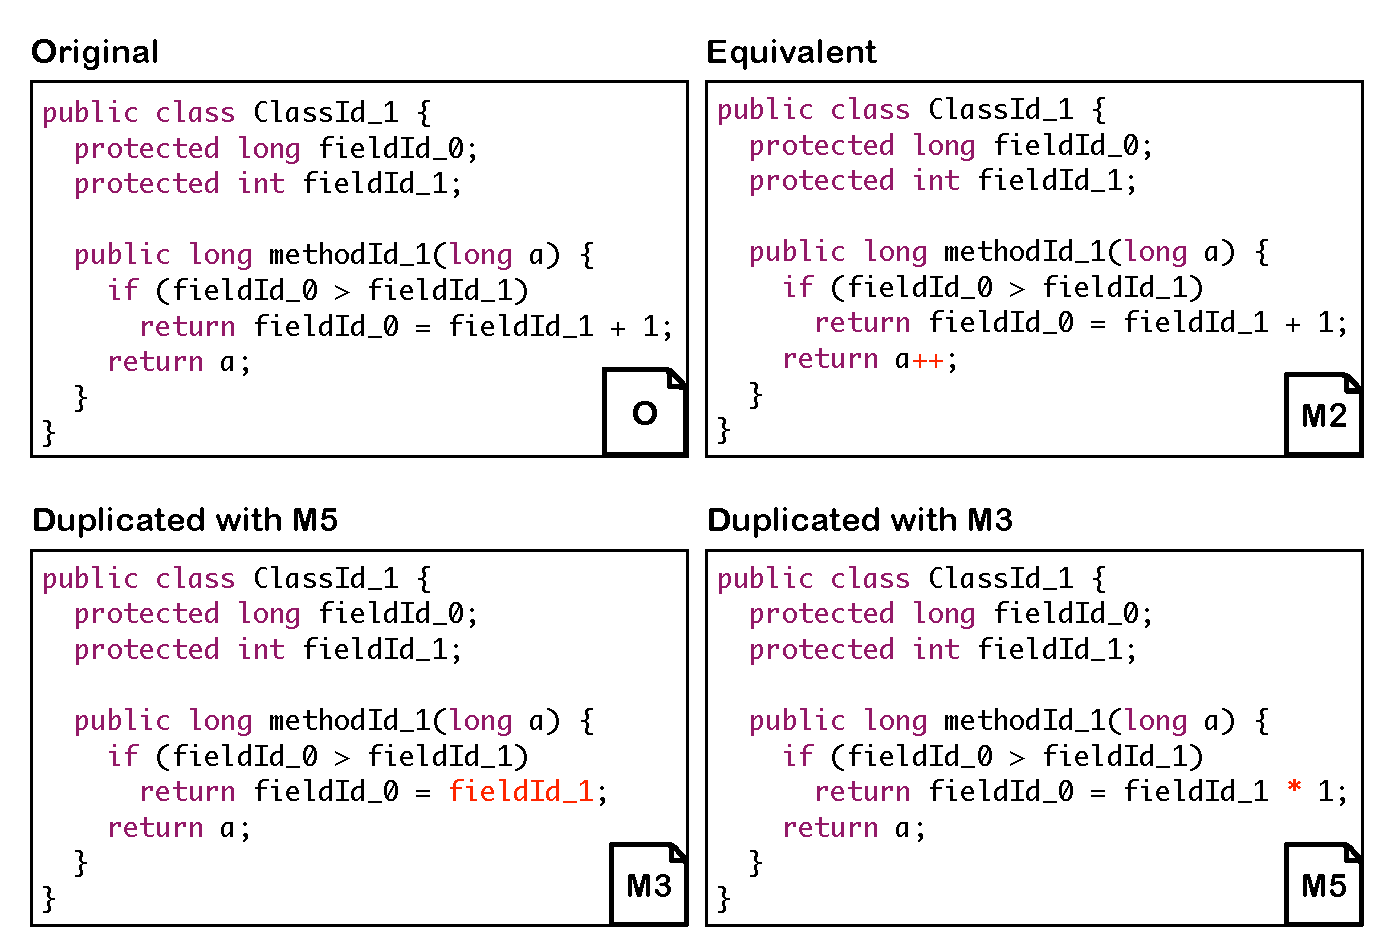
\includegraphics[scale=0.5]{images/Background.pdf}
\caption{Original program and three mutants.}
\label{fig:background}
\end{center}
\end{figure}

Previous work~\cite{MADEYISKI:2014:1} reported that the rate of equivalent mutants might lie between 4\% and 39\%. 
In addition, manually checking mutant equivalence is error-prone (people judged equivalence correctly in about 80\% of the cases~\cite{ACREE:1980:1}) and time consuming (approximately 15 minutes per equivalent mutant~\cite{SHULER:2013:1}). 
Recently, duplicated mutants have been discussed and tackled. 
Researchers reported 21\% of duplicated mutants in their empirical study~\cite{KINTIS:2017:1}.

In this work, we introduce a strategy to help with identifying rules capable of avoiding useless mutants. 
To use the strategy, we need a set of programs as input. 
In addition, for each program in this set, the strategy also needs a green test suite and a set of mutants derived from the program. 
The strategy then runs every test against every mutant and yields equivalent and duplicated mutants candidates. 
Our strategy is flexible in the sense we can instantiate it with different programs and their respective test suites. To generate the mutants, we can instantiate the strategy with different mutation testing tools.

% As you can see, our strategy works similarly to a normal mutation analysis.
% But we use the test suite itself to identify useless mutants.
% It is based on three major modules that are flexible to instantiate one or more tools for each one of the modules.

% \begin{itemize}
%     \item The program input.
%     \item The mutants.
%     \item The test suite.
% \end{itemize}

To classify the mutants as equivalents or duplicated, the strategy proceeds as follows. 
Given a program \textit{P}, when its test suite \textit{T} is executed in a mutant \textit{M} and it does not have any failing test case, the strategy classifies \textit{M} as an equivalent mutant candidate. If two mutants \textit{M$_i$} and \textit{M$_j$} have the same non-empty set of failing test cases in \textit{T}, the strategy classifies \textit{M$_i$} and \textit{M$_j$} as duplicated mutants candidates. 

To evaluate our strategy, we instantiate it with programs automatically generated by the \jdolly{} program generator~\cite{SOARES:2013:1}. 
\jdolly{} exhaustively generates programs up to a given scope. 
It encodes a metamodel for Java and uses the Alloy specification language \cite{alloy-book} to find possible solutions, which are translated into Java programs.
The user can specify constraints to guide \jdolly{} to generate programs in a given scope.
In our work, we set \jdolly{} to generate \AnalyzedPrograms programs with few Java constructs. 
This reduced Java scope makes the task of deriving rules to avoid useless mutants easier. 

As our programs did not have any test suite, we use \randoop{}~\cite{PACHECO:2007:1} to automatically
generate unit tests for the classes and methods received as parameters within a time limit.
A unit test generated by \randoop{} typically consists of a sequence of
method and constructor invocations that create and mutates objects with random values and a JUnit assertion.

%\todo{Last but not least}, 
%we choose to work in Java since it is widely used by practitioners and forms the subject of most of the recent research papers.
To generate the mutants, we instantiate three of the most used Java mutation testing tools, i.e., \mujava{}~\cite{OFFUTT:2005:1, OFFUT:2006:1}, \major{}~\cite{JUST:2011:1}, and \pit{}~\cite{PIT:2017}.
These tools, in addition to being the most used in previous research, bring different mutation operators as well as different approaches to mutant generation: source code mutation (\mujava{}), byte code mutation (\pit{}), and compiler-integrated mutation (\major{}).

The three mutation testing tools generated 4,999 mutants. 
The strategy classified 963 as equivalent and 1,332 as duplicated.
By analyzing the results, we observe we could avoid many mutants classified as useless in case we perform an analysis of the context in which the mutation is applied.
We can retrieve this context by navigating throughout the Abstract Syntax Tree (AST) or by using \textit{def-use} analyses.
So, the output of our strategy is important because it enables us to derive rules to avoid the generation of these mutants. 

In particular, after manually analyzing the output, we derived \NumberOfIdentifiedHeuristics rules. 
To the best of our knowledge, \NumberOfNewHeuristics out of \NumberOfIdentifiedHeuristics are first introduced in this work.
%A rule is defined as a triple ($terms$, $transformations$, $constraints$).
%This small set of information, which we better explain each part in Chapter \ref{sec:rules}, is sufficient to predict some useless mutants and thus prevent them from being generated.
To evaluate the effectiveness of our rules on reducing costs, we have implemented a subset of them in the \mujava{} tool. 
We execute the tool using classes of well-known projects such as \textit{ant}, \textit{bcel}, and \textit{commons-lang}. 
As results, we reduce the number of mutants by almost 13\% on average, demonstrating potential. 
One might wonder that this number is low when compared to related work. 
However, these results are promising because differently from previous work~\cite{PAPADAKIS:2015:1, KINTIS:2017:1, BALDWIN:1979:1, OFFUT:1996:1, OFFUT:1997:1, VOAS:1997:1, HIERONS:1999:1, GRUN:2009:1, SHULER:2010:1, SHULER:2013:1, SHULER:2009:1}, we do \textit{not} generate, compile, and analyze whether the mutants are useless or not. 
Instead, we avoid them: our rules are capable of discarding such mutants right before their generation. Also, we can derive more rules in case we set our strategy with more complex Java programs. Last but not least, we have implemented only a subset of our rules. We focused on rules that do not need \textit{def-use} analyses. 

We also calculated the execution time of our rules to better understand whether pre-analyzing and avoiding mutants is faster than generating useless mutants and checking whether they are indeed useless or not. Despite the overhead introduced by our rules, the payoff amount is higher than 12\% for all projects we considered in this work and reached almost 20\% in two projects.

%An important issue arises when we add an overhead before generating mutants. Would it be better to generate the useless mutants and then detect them instead of doing a pre-analysis to avoid them? After all, although we avoid some mutants, these rules would be executed every time that mutation operator is selected. To understand this trade-off, we calculate the execution time of the tool either without the rules and with the rules embedded. To our surprise, despite the overhead introduced by our rules, the payoff amount is higher than 12\% for all projects and reached almost 20\% in two projects which we analyzed. That is, the cost of running all rules is offset by the decrease in the number of mutants to generate and compile.

This work presents the following contributions:

\begin{itemize}
    
    \item A strategy to help with identifying rules to avoid equivalent and duplicated mutants (Chapter~\ref{sec:strategy});
    
    \item We introduce \NumberOfNewHeuristics new rules to \textit{avoid} the generation of equivalent and duplicated mutants (Chapter~\ref{sec:rules});
    
    \item We provide a \mujava{} implementation embedded with \NumberOfImplementedHeuristics implemented rules (Chapter~\ref{sec:implementing}).
    
    \item An empirical study to evaluate our rules. In particular, we avoid almost 13\% (on average) of useless mutants in classes of well-known projects such as \textit{ant}, \textit{bcel}, and \textit{commons-lang} with a payoff amount higher than 12\% for all projects in the execution time (Chapter~\ref{sec:implementing});
    
\end{itemize}


%\section[Motivation  (Why to Automate CR Assignment?)] {Motivation (Why to Automate \ac{cr} Assignment?)}
%\label{sec:intro-motivation}
%
%\section{Problem Statement}
%\label{sec:intro-problem-statement}
%
%\section{Overview of the Proposal}
%\label{sec:intro-solution}
%
%\section{Research Methodology}
%\label{sec:intro-methodology}

%This research design of this thesis is based on a multimethod
%approach~\citep{Hesse-Biber2010}. Such approach combines two or more
%quantitative (or qualitative) methods in a single study, such as a survey and an
%experiment~\citep{Hesse-Biber2010}. Multimethod must not be confused with mixed
%method. In this last, methods for both qualitative and quantitative types of
%research are applied in a single study. On the other hand, multimethod studies
%combine different methods for a single research type.
%
%When applying a multimethod approach, the triangulation is used to consolidate
%the results from the different methods, considering, however, that the same
%research question(s) was/were investigated in these methods. As a consequence,
%the triangulation of methods enhances the conclusions and completeness of the
%study, bringing more credibility to the research
%findings~\citep{Hesse-Biber2010}. \figref{fig:research-methodology-thesis} shows
%the multimethod research design applied in this thesis.
%
%\begin{figure}[h]
%\centering
%  \caption[Research methodology.]{The research methodology applied for this
%  thesis.}
%  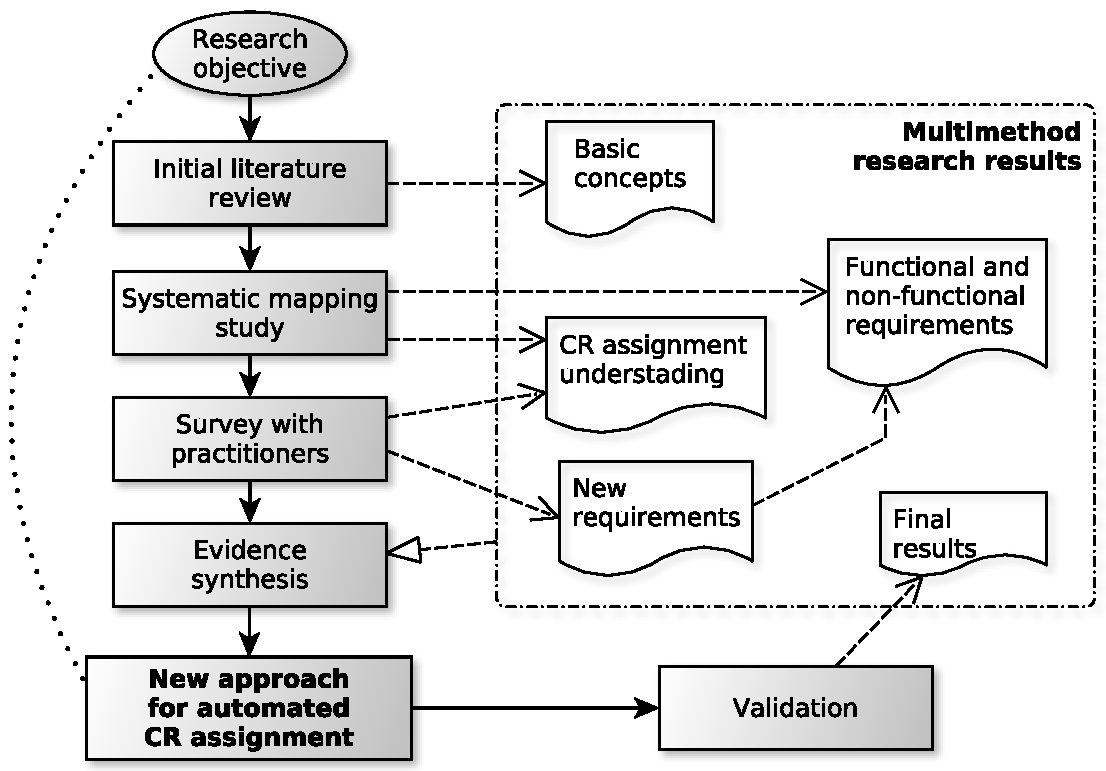
\includegraphics[width=\columnwidth]{images/research-methodology-thesis.pdf}
%  \footnotesize{Source: Made by the author.}
%  \label{fig:research-methodology-thesis}
%\end{figure}
%
%The design started by stating the research objective, which we defined in
%\secref{sec:intro-problem-statement}, and performing the initial literature
%review. This last provided the basic concepts and understanding of the area.
%Then, a systematic mapping study and a questionnaire-based survey were
%conducted. These two gathered detailed information on our research topic.
%Indeed, both of them were used to understand the key aspects of \ac{cr}
%assignment and identify the set of requirements to automate the assignments. In
%the evidence synthesis step, these results were detailed and organized in order
%to formulate the approach to automate \ac{cr} assignments, which was constructed
%in the next step. Finally, the research design states the validation of the
%proposed approach.

%\section{Out of Scope}
%\label{sec:intro-outofscope}
%As the proposed approach is part of a broader context, a set of related aspects will be left out of its scope. Thus, the following topics are not directly addressed in this thesis:
%
%\begin{enumerate}
%  \item \textbf{Tools for \ac{cr} management.} We are addressing
%  a specific aspect of \ac{cr} management, which is the \ac{cr} assignment
%  activity. Thus, it is out of scope of this thesis to provide a
%  complete solution for \ac{cr} management. Instead, we are planning to
%  implement standalone software which will be able to integrate with the
%  most well known tools for \ac{cr} management, such as Mantis, Bugzilla, and
%  Trac, providing a service to leverage the automation of \ac{cr}
%  assignments.
%  
%  \item \textbf{Software maintenance process.} Software maintenance involves
%  a set of activities aiming at implementing modifications in some software
%  project. These activities must be coordinated through a process so that the
%  maintenance can be successful. In Chapter 2, we discuss some of
%  these processes. However, in this thesis, we are not concerned with the
%  maintenance process itself. Actually, it should be transparent in our approach
%  to automate \ac{cr} assignment. Thus, it is out of scope of this
%  thesis to provide any process assessment for software maintenance beyond the
%  activity of \ac{cr} assignment.
%  
%  \item \textbf{\ac{ir} models.} Many models for \ac{ir} have been proposed for
%  different objectives, including the \ac{cr} assignment itself. However, due to
%  the broad availability of these models, it is out of scope of this thesis to
%  develop a new one. Instead, the \ac{ir} models with better performance,
%  identified through the systematic mapping study, were chose to be
%  integrated in our approach;
%  
%  \item \textbf{Rule-based expert systems.} Similar to \ac{ir} models,
%  rule-based expert systems have a long history of development. Thus, our
%  approach does not intend to develop a whole new system with this purpose.
%  Actually, we integrated in our approach the
%  Drools\footnote{\url{http://www.jboss.org/drools/}} expert system, which is a
%  mature tool that can be easily manipulated;
%  
%  \item \textbf{Mathematical formulations on NP-Complete problems.} We
%  understand that the problem of assigning \acp{cr} to software developers is in
%  the broad category of \emph{assignment problems}, which is well known to be
%  NP-Complete. Thus, could be formulated as such. However, the mathematical
%  formulations of the \ac{cr} assignment problem is out of scope of this thesis.
%  As well as finding an optimal solution on the context of NP-Complete problems
%  is also out of scope. The main reason for this is the human factors and
%  context variables that are involved in the assignment of \acp{cr}, which
%  make this problem hard to be computable. A mathematical formulation of the
%  \ac{cr} assignment problem is provided by~\citet{Rahman2009}.
%\end{enumerate}

%\section{Statement of the Contributions}
%\label{sec:intro-contibutions}

%\section{Organization of the Thesis}
%\label{sec:intro-organization}


\chapter{Background}
\label{chp:background}

This chapter exposes the concepts of mutation testing and the problem of useless mutants. 
%In addition, we come up with concepts related to our strategy in special the technologies we instantiate for conduct the experiments. 
%In spite of being succinct, this summary suffices for the purposes of this work. A more precise introduction of mutation testing can be found in \cite{JIA:2011:1, DEMILLO:1978:1, OFFUTT:2001:1, WOODWARD:1993:1}. 
The rest of the chapter is organized as follows: we introduce mutation testing concepts through the process analysis, the importance of design good mutation operators, examples of mutation tools, and the associated cost of the technique. Thereafter we bring the problem of useless mutants up and how we can overcome it. 

\section{Mutation Testing}
Mutation Testing is a fault-based technique: it injects artificial faults into software by creating many copies of the original program, each one containing one (or more) simple fault(s). 
Then it executes the test suite against these copies to check the compliance of the output from that of the original program. 

Mutation Testing has been increasingly studied since it was first proposed in the 1970s \cite{LIPTON:1971:1, DEMILLO:1978:1}. 
Many research papers have appeared on several points of the mutation process seeking to turn Mutation Testing into a practical approach. 

We detail this process in what follows, indicating the automatic and manual parts.

\subsection{The Mutation Analysis Process}
The main aim of mutation testing is adequacy measurement of a test set. 
For this, some steps need to be taken. 
Offutt and Untch \cite{OFFUTT:2001:1} establishes a generic mutation testing process. We illustrate this process in Figure \ref{fig:mutation_process}. 

\begin{figure}[h]
	\centering
	\caption{Mutation Testing Process}
	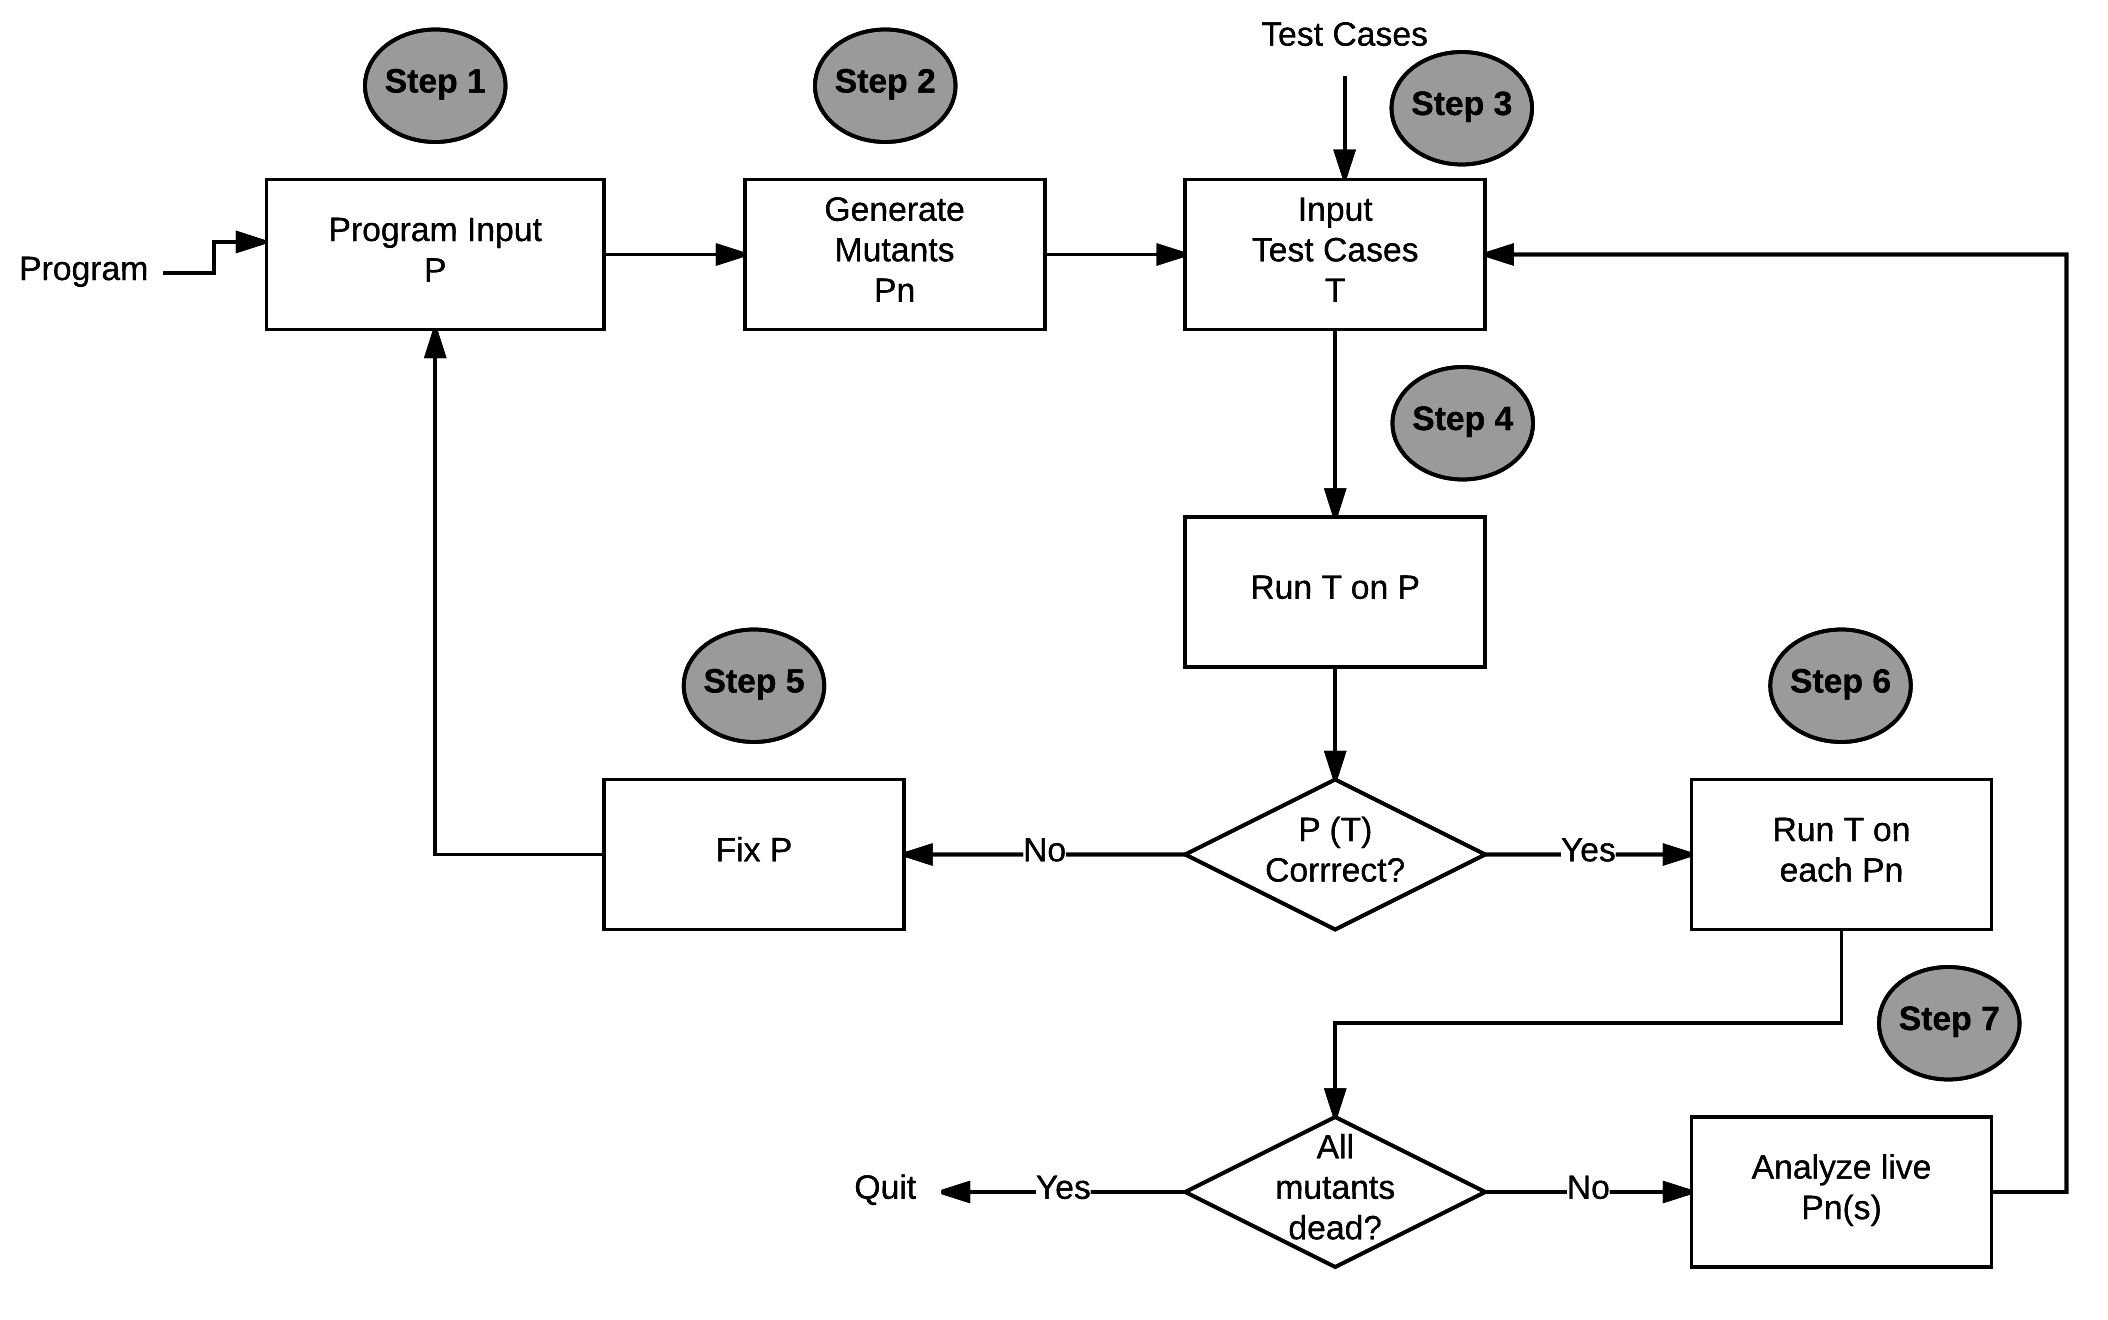
\includegraphics[scale=0.8]{images/mutation-testing-process.png}
	\label{fig:mutation_process}
\end{figure}

Based on an original program input $P$ provided by the developer (Step 1), the mutation testing tool generates a set of faulty programs $Pn$, called \textit{mutants}, by making small syntactic changes from the original program $P$ (Step 2). 
%Figure \todo{...} shows examples of mutations for common statements in imperative languages. 
In the next step, a test set $T$ is supplied to the system (Step 3), and we run $T$ on $P$ (Step 4). 
In case $T$ detects an error in $P$ it is necessary to fix $P$ and start over (Step 5).
But if no error is detected in $P$, the mutation testing tool executes the test set $T$ against each mutant $Pn$ and check its correctness (Step 6). 
If the result of running $Pn$ is different from the result of running $P$ for at least one test case in $T$, then the mutant $Pn$ is said to be ``\textit{killed}'', otherwise it is said to have ``\textit{survived}''.
In case all mutants have been killed so the process ends, but if there is surviving mutants, the developer analyzes these mutants to mark the equivalent mutants (explained in Section \ref{sec:useless_mutants}) or to improve the test suite to kill the mutants that are still alive (Step 7).

Steps 2, 4 and 6 are executed automatically by the majority of the mutation testing tools. 
Steps 1, 3, 5 and 7 need a manual intervention.

The mutation testing tool concludes with an adequacy score to indicate the quality of the test set $T$. The most common adequacy score is the \textit{mutation score}. It is the ratio of the number of killed mutants over the total number of mutants minus the total of equivalents. 

\[ MS=\frac{Mk}{Mt - Me} \]

Where $Mt$ is the total number of produced mutants, $Mk$ is the number of killed mutants and $Me$ is the number of equivalent mutants.
The final value of the mutation score ranges between zero and one, so the closer to one indicates a better result.

When we talk about killing, the way a mutant is killed during the execution process can be classified into three types: \textit{strong}, \textit{weak}, and \textit{firm mutation}. 
%Strong Mutation is often referred to as traditional Mutation Testing \todo{citar 66}. 
% In Strong Mutation, for a given program $P$, a mutant $Pn$ of program $P$ is said to be killed only if mutant $Pn$ gives a different output from the original program $P$.
% In Weak Mutation \todo{citar 115}, instead of checking mutants after the execution of the entire program (or until call the proper output), the mutants need only to be checked immediately after the execution point of the mutant or mutated component.
    % That is, once the mutated component is executed we can check its internal state immediately after the execution of the mutated components and compare with the original program.

In weak mutation~\cite{HOWDEN:1982}, a test kills a mutant if the test execution leads to a difference between the program state of the mutant and the program state of the original version immediately after the execution of the mutated point. 
In contrast, strong mutation~\cite{DEMILLO:1978:1}, often referred to as traditional mutation testing, requires that this difference propagates to an observable output, i.e., an assertion failure or an exception.
Weak mutation is less computationally expensive than strong mutation since we just need to execute the test until the mutated point.
However, given that it is easier to kill weak mutants, then we will sacrifices test effectiveness for improvements in test effort.
This raises the question as to what kind of trade-off can be achieved.
The idea of firm mutation~\cite{WOODWARD:1988:1} is to overcome the disadvantages of both weak and strong mutations by providing a continuum of intermediate possibilities. 
That is, the ``compare state'' of firm mutation lies between the intermediate states after execution (weak mutation) and the final output (strong mutation).
To the best of our knowledge, there is no publicly available firm mutation tool.
In this work, we use the traditional idea of killing a mutant using strong mutation.

In the next section we take a look at the first automated step (Step 2) of a mutation tool. 
The generation of the mutants.

\subsection{Mutants Creation}
Mutants contain faults that are simple syntactic changes based on specific rules known as \textit{mutation operators}. 
Typical mutation operators are designed to modify variables and expressions using replacement, insertion or deletion operators. 
The first objective of a mutation operator is to mimic typical faults that programmers can commit, such as using the wrong operator or omitting a statement.
And the second objective is forcing tests that are usually considered valuable, such as forcing expressions to have the value zero or forcing the execution of all paths in a conditional statement.

The design of mutation operators is crucial to the success of the mutation tool.
The tool must generate as few mutants as possible without losing effectiveness, which means to simulate the maximum number of bugs, but, preferably without incurring in duplicated mutants.
Generate hard-to-kill mutants (also known as stubborn mutants \cite{YAO:2014:1}) help developers to improve their test suite and trivial-to-kill mutants offers no benefits, however, this task is not trivial. 
Besides that, the operators are very dependent on the programming language of choice. For example, the set of operators for Java must be different for the set of operators for Haskell, since the errors that programmers of these languages make tend to be different. 

When a mutant is created by changing one single code location we say it is a \textit{first order mutant}. 
In case the mutant is generated changing more than one place we say it is a \textit{high order mutant} \cite{JIA:2008:1}. 
%\textit{Second order mutants} are the most common \textit{high order mutant}, however 
Tools that implement high order mutants are still scarce \cite{MADEYISKI:2014:1}. 
In this work, we use tools that create first order mutants.
%X and Y \todo{Ref. revisao de mut. equiv.} proposed different algorithms to combine \ac{fom} to generate the second order ones.

\subsection{Mutation Testing Tools}
To make the use of the mutation technique possible, we need tools.
In this work we have selected the following tools to generate the mutants:
\mujava{}~\cite{OFFUTT:2005:1, OFFUT:2006:1}, \major{}~\cite{JUST:2011:1}, and \pit{}~\cite{PIT:2017}.

\mujava{} (Mutation System for Java) \cite{OFFUTT:2005:1, OFFUT:2006:1}, is one of the oldest Java mutation testing tools and has been used in many mutation testing studies. 
The tool manipulates the source code of the program under test and supports two types of mutation operators: class-level and method-level. 
The class-level mutation operators were designed for Java classes and it handles object-oriented specific features such as inheritance, polymorphism, and dynamic binding \cite{MA:2002:1, OFFUT:2006:1}. 
Method-level (traditional) mutants are based on the selective operator set by Offutt et al. \cite{OFFUT:1996:1} and it handles primitive features of the languages.
%Table \todo{montar tabela} presents the operators of the tool, along with a succinct description of the performed changes.
After creating mutants, \mujava{} allows the tester to enter and run tests automatically.
Equivalent mutants must be identified by hand.
In April 2015, \mujava{} has been released as open source under the Apache license.\footnote{\url{https://github.com/jeffoffutt/MUJAVA}}

%Artigo Kintis compara as ferramentas e site
\pit{} \cite{PIT:2017} is a mutation testing framework that targets primarily the industry but has also been used in many research studies.
%Table \todo{Table PIT} describes the corresponding operators. 
%By comparing this table with Table \todo{Tabela MUJAVA}, it can be seen that PIT implements differently specific mutation operators of MUJAVA, for instance, the changes imposed by PIT's Conditionals Boundary operator are a subset of the ones of MUJAVA's Relational Operator Replacement (ROR). 
%Additionally, it employs mutation operators that are not implemented in MUJAVA, e.g. the Void Method Calls and Constructor Calls operators.
\pit{} mutates the bytecode, i.e, it does not compile the code but instead modifies the byte code in memory and \pit{} only requires the location of the source code in order to generate a human readable report.
It employs mutation operators that affect primitive programming language features.
For this work, we extend \pit{} to write all generated mutants in the disk. 
This is important to the equivalent and duplicated analysis. 
\pit{} has been released as open source under the Apache license.\footnote{\url{https://github.com/hcoles/pitest}}

%Artigo Kintis compara as ferramentas e paper sobre a ferramenta
\major{} \cite{JUST:2011:1} is integrated into the Java compiler, in a non-invasive way, and does not require a specific mutation analysis framework. 
The tool manipulates the AST of the program under test. 
The implemented mutation operators are based on a reduced set of operators defined by Offutt et al. \cite{OFFUT:1996:1}, similarly to \mujava{}.
%Table \todo{montar tabela MAJOR} summarizes \major{}'s operators and their imposed changes. 
%As observed by \cite{Kintis:2016}, compared to MUJAVA's operators, it is evident that the two tools share many mutation operators, but implement them differently. 
%Compared to PIT, most operators of MAJOR impose a superset of changes with respect to the corresponding ones of PIT and there are operators of PIT that are completely absent from MAJOR.
\major{} uses mutant schemata \cite{UNTCH:1993:1}. 
That is, to reduce the number of generated versions it produces a \textit{metaprogram} that is derived from the program under study and contains multiple mutations.
Each mutation is guarded by a conditional statement that can be switched on and off at runtime.
To use the mutant for further equivalence analysis, the tool exports each generated mutant to an individual source-code file.
\major{} can be downloaded for free, but does not have its source code released.\footnote{\url{http://mutation-testing.org/}}
%end of the tool explanation

Although they are very mature tools, they do not have embedded solutions to solve some of the inherent cost problems of mutation testing.
%The literature reviews about this theme \cite{JIA:2011:1, MADEYISKI:2014:1} demonstrated a  growing academic interest in mutation testing over the years and its expansion to a vast number of platforms/languages. 
%However, this same interest has not been accompanied by industry, mainly because of the cost barrier. 
In the last years solutions have been proposed to reduce the cost of use mutation testing in real world scenarios. 
We now check some of them.

\subsection{Cost Reduction Techniques}
The barriers that prevent the practical use of mutation testing can be classified into two groups: computational cost and manual labor cost.

The major computational cost of mutation testing arises from the high number of generated mutants and the high computing time to execute each mutant.
Offut and Untch \cite{OFFUTT:2001:1} classify three strategies to solve this problem: \textit{do fewer}, \textit{do faster}, and \textit{do smarter}. 
The ``do fewer'' approaches try to decrease the number of mutants generated without losing effectiveness. 
The ``do faster'' approaches focus on ways of generating and running the mutants as quickly as possible. 
The ``do smarter'' approaches look for clever solutions to generate and run mutants, such as running only the test cases that are necessary for each mutant or distribute the computational expense over several machines. 
%Table \todo{fazer tabela com solucoes} brings the last solutions to computational cost reduction.
For a more detailed list of advances in this field, please refer to \cite{JIA:2011:1, OFFUTT:2001:1}.

% \scriptsize
% \begin{table}
% 	\caption{...}
% 	\centering
% 	\begin{tabular}{|c|c|c|}
% 		\hline
% 		\textbf{Approach} & \textbf{Description} & \textbf{References} \\
% 		\hline
% 		X & Y & Z \\
% 		\hline
% 	\end{tabular}
% 	\label{tab:solutions_computational_cost}
% \end{table}
% \normalsize

In a recent work, Papadakis et al. \cite{PAPADAKIS:2015:1} highlight the problem of \textit{duplicated mutants}. 
That is, two mutants that are equivalent to each other, even if they are not equivalent to the original program from which they are constructed; either one or the other of these two mutually equivalent mutants can be discarded, saving some effort. 
This work tackles this problem and it is better discussed in the next section.

The other side of the cost problem comes from the manual labor cost, i.e. the amount of human effort involved to do some tasks. 
The first one is also known as the \textit{Human Oracle Problem} and claim that the developer needs to know the program's output to assert a testing criterion. 
This problem is inherent to all forms of testing. 
Advances in automatic test case generation can support this laborious task. 
The second one is the Equivalent Mutant Problem. 
Although syntactically different from the original program, the mutant can be semantically equal, which implies that their behavior does not change to any input data, thus the developer needs to check whether a survived mutant is merely hard to kill (one more test case is necessary) or equivalent (no test can kill it, so any attempt will be futile).

This work focuses on the problems of equivalent and duplicated mutants, which \cite{PAPADAKIS:2015:1} names as \textit{useless mutants}. 
The next section explains in more detail the problem of useless mutants.

\section{Useless Mutants}
\label{sec:useless_mutants}
We use the term \textit{useless} to represent equivalent and duplicated mutants. 
These mutants do not incorporate anything to the mutation testing process \cite{PAPADAKIS:2015:1}. 

Equivalent mutants, as explained, occur when the mutant maintains the same behavior as the original program. 
It is a well-known impediment to the practical adoption of mutation testing. 
Budd and Angluin \cite{BUDD:1982:1} have already proven that this is an undecidable problem in its general form. 
Thus, no complete automated solution exists. 
To worsen the situation, manually detecting equivalent mutants is an error-prone and time-consuming task. 
Acree~\cite{ACREE:1980:1} showed that 20\% of the studied mutants were erroneously classified, i.e., a killable mutant classified by mistake as equivalent or vice versa. 
Shuler et al.~\cite{SHULER:2013:1} showed that developers take, on average, 15 minutes to manually classify a mutant as equivalent or nonequivalent.
This problem becomes quite relevant when empirical studies report that between 10\% and 40\% of all the generated mutants are equivalent \cite{OFFUTT:1994:1, OFFUT:1997:1}.
So solutions, even partial, can greatly help reduce this cost.
%Even though it is an undecidable problem, partial semi-automated solutions have been proposed to diminish its adverse effects. 
%The work of Madeyiski et al.~\cite{MADEYISKI:2014:1} surveyed those solutions \todo{and identified 17 relevant techniques (in 22 articles).}

%...and classified in three categories of techniques to solve this problem: \textit{Detecting}, \textit{Suggesting}, and \textit{Avoiding}. 
%The Table \todo{...} shows those solutions.
%\todo{Continuar...}.

Duplicated mutants are a more recent problem \cite{PAPADAKIS:2015:1, KINTIS:2017:1}. 
That is, if the mutant $P1$ is duplicated to the mutant $P2$, all the tests that kill $P1$ \textit{are exactly the same} that kill $P2$.
Although it does not involve a manual effort as equivalent mutants, duplicated mutants take a worthless computational cost, given that the test set needs to execute against two or more mutants that have the same behavior.
Papadakis et al.~\cite{PAPADAKIS:2015:1} was able to detect 21\% of the mutants as duplicated, however this number may be even higher, since the technique proposed by Papadakis does not detect all cases.
Besides the cost, duplicated mutants make the mutation score imprecise as reported by Kutz et al. \cite{KURTZ:2016:1}. 
For example: Consider a set of 10 nonequivalent mutants $M$ and a set of 10 tests $T$. 
If we execute $T$ against $M$ and it kills 7 mutants, the mutation score is 0.7. 
If 10 more mutants are added to $M$, but all of them are duplicated with a some previous mutant in the set.
That is, there are 20 nonequivalent mutants and 17 are killed, thus the mutation score is now 0.85.
This shows that without any improvement in the test suite the value of the mutation score has changed.
This example and the high number of duplicated mutants that can be generated highlight the importance of having solutions to reduce this problem.

Our work focuses on avoiding useless mutants before they are generated.
In Chapter \ref{sec:strategy} we come up with a strategy to support mutation tool developers to derive rules to avoid useless mutants. 
We show some of these rules in Chapter~\ref{sec:rules} and evaluate them in Chapter~\ref{sec:implementing}.

% \section{Research Status}
% We have included a section on the next steps at the end of all the chapters that follow.
% Here we list what we intend to do about the Background chapter.
% In the Concluding Remarks chapter, we present a schedule for each task.

% \begin{enumerate}
%     \item We plan to extend this chapter by including more details and examples of each concept we use throughout this work.
%     \item We might include examples of common transformations for imperative languages, in special for Java constructs.
%     \item Moreover, we intend to include a list of all mutation operators from the tools we use throughout this work.
%     \item We could also include a table summarizing the main solutions that address the problem of equivalent and duplicated mutants.
%     \item Finally, we plan to extend the Section \ref{sec:useless_mutants} with the redundant mutants that are a more general form of duplicated mutant. 
% \end{enumerate}








%\section{Automated Testing Generation}
%\todo{...}

%\section{Alloy}
%\todo{...}





\chapter{Strategy}
\label{sec:strategy}

In this chapter, we present our strategy that helps with the identification of rules to avoid the generation of useless mutants. 
We explain the strategy in Section~\ref{sec:strategy-identifying}. 
Then, we evaluate the strategy in Section~\ref{sec:strategy-evaluation}.
Finally, we discuss the research status in Section~\ref{sec:research-status-strategy}


\section{Identifying Useless Mutants Candidates}

\label{sec:strategy-identifying}

Our strategy is based on three inputs. 
The first one comprises a set of programs. 
For each program, the strategy also needs a green test suite and a set of mutants. 
Figure~\ref{fig:strategy} illustrates the strategy. 
First, we collect the set of programs (Step~1). 
Steps~2 and~3 collect a passing test suite and a set of mutants for each program of the Step~1. 
For each mutant gathered in Step~3, we execute all tests of Step~2 and collect the results (Step~4). 
In the last step, we identify potential candidates of equivalent and duplicated mutants (Step~5).

To classify the mutants as equivalents or duplicated candidates, the strategy proceeds as follows. 
Given a program \textit{P}, when its test suite \textit{T} is executed in a mutant \textit{M} (generated from \textit{P}) and \textit{T} does not have any failing test case, \textit{M} seems to not change the behavior of the original program \textit{P}. 
This way, the strategy sets \textit{M} as an equivalent mutant candidate. 
If two mutants generated from \textit{P} (\textit{M$_i$} and \textit{M$_j$}) have the same non-empty set of failing test cases in \textit{T}, the strategy sets \textit{M$_i$} and \textit{M$_j$} as duplicated mutants.

We are classifying mutants as useless or useful according to \textit{strong kill}, that is, for a given program \textit{P}, a mutant \textit{M} of program \textit{P} is said to be killed only if mutant \textit{M} gives a different output from the original program \textit{P}.

Notice that our strategy is flexible in the sense we can collect programs, test suites, and mutants from different tools and setups. 
In Figure~\ref{fig:strategy}, we illustrate the strategy using a program generator named \jdolly{}~\cite{SOARES:2013:1}, a test suite generator (\randoop{}~\cite{PACHECO:2007:1}), and a mutation testing tool to generate mutants of a given program, e.g., \pit{}~\cite{PIT:2017}.

\begin{figure*}[ht]
	\begin{center}
		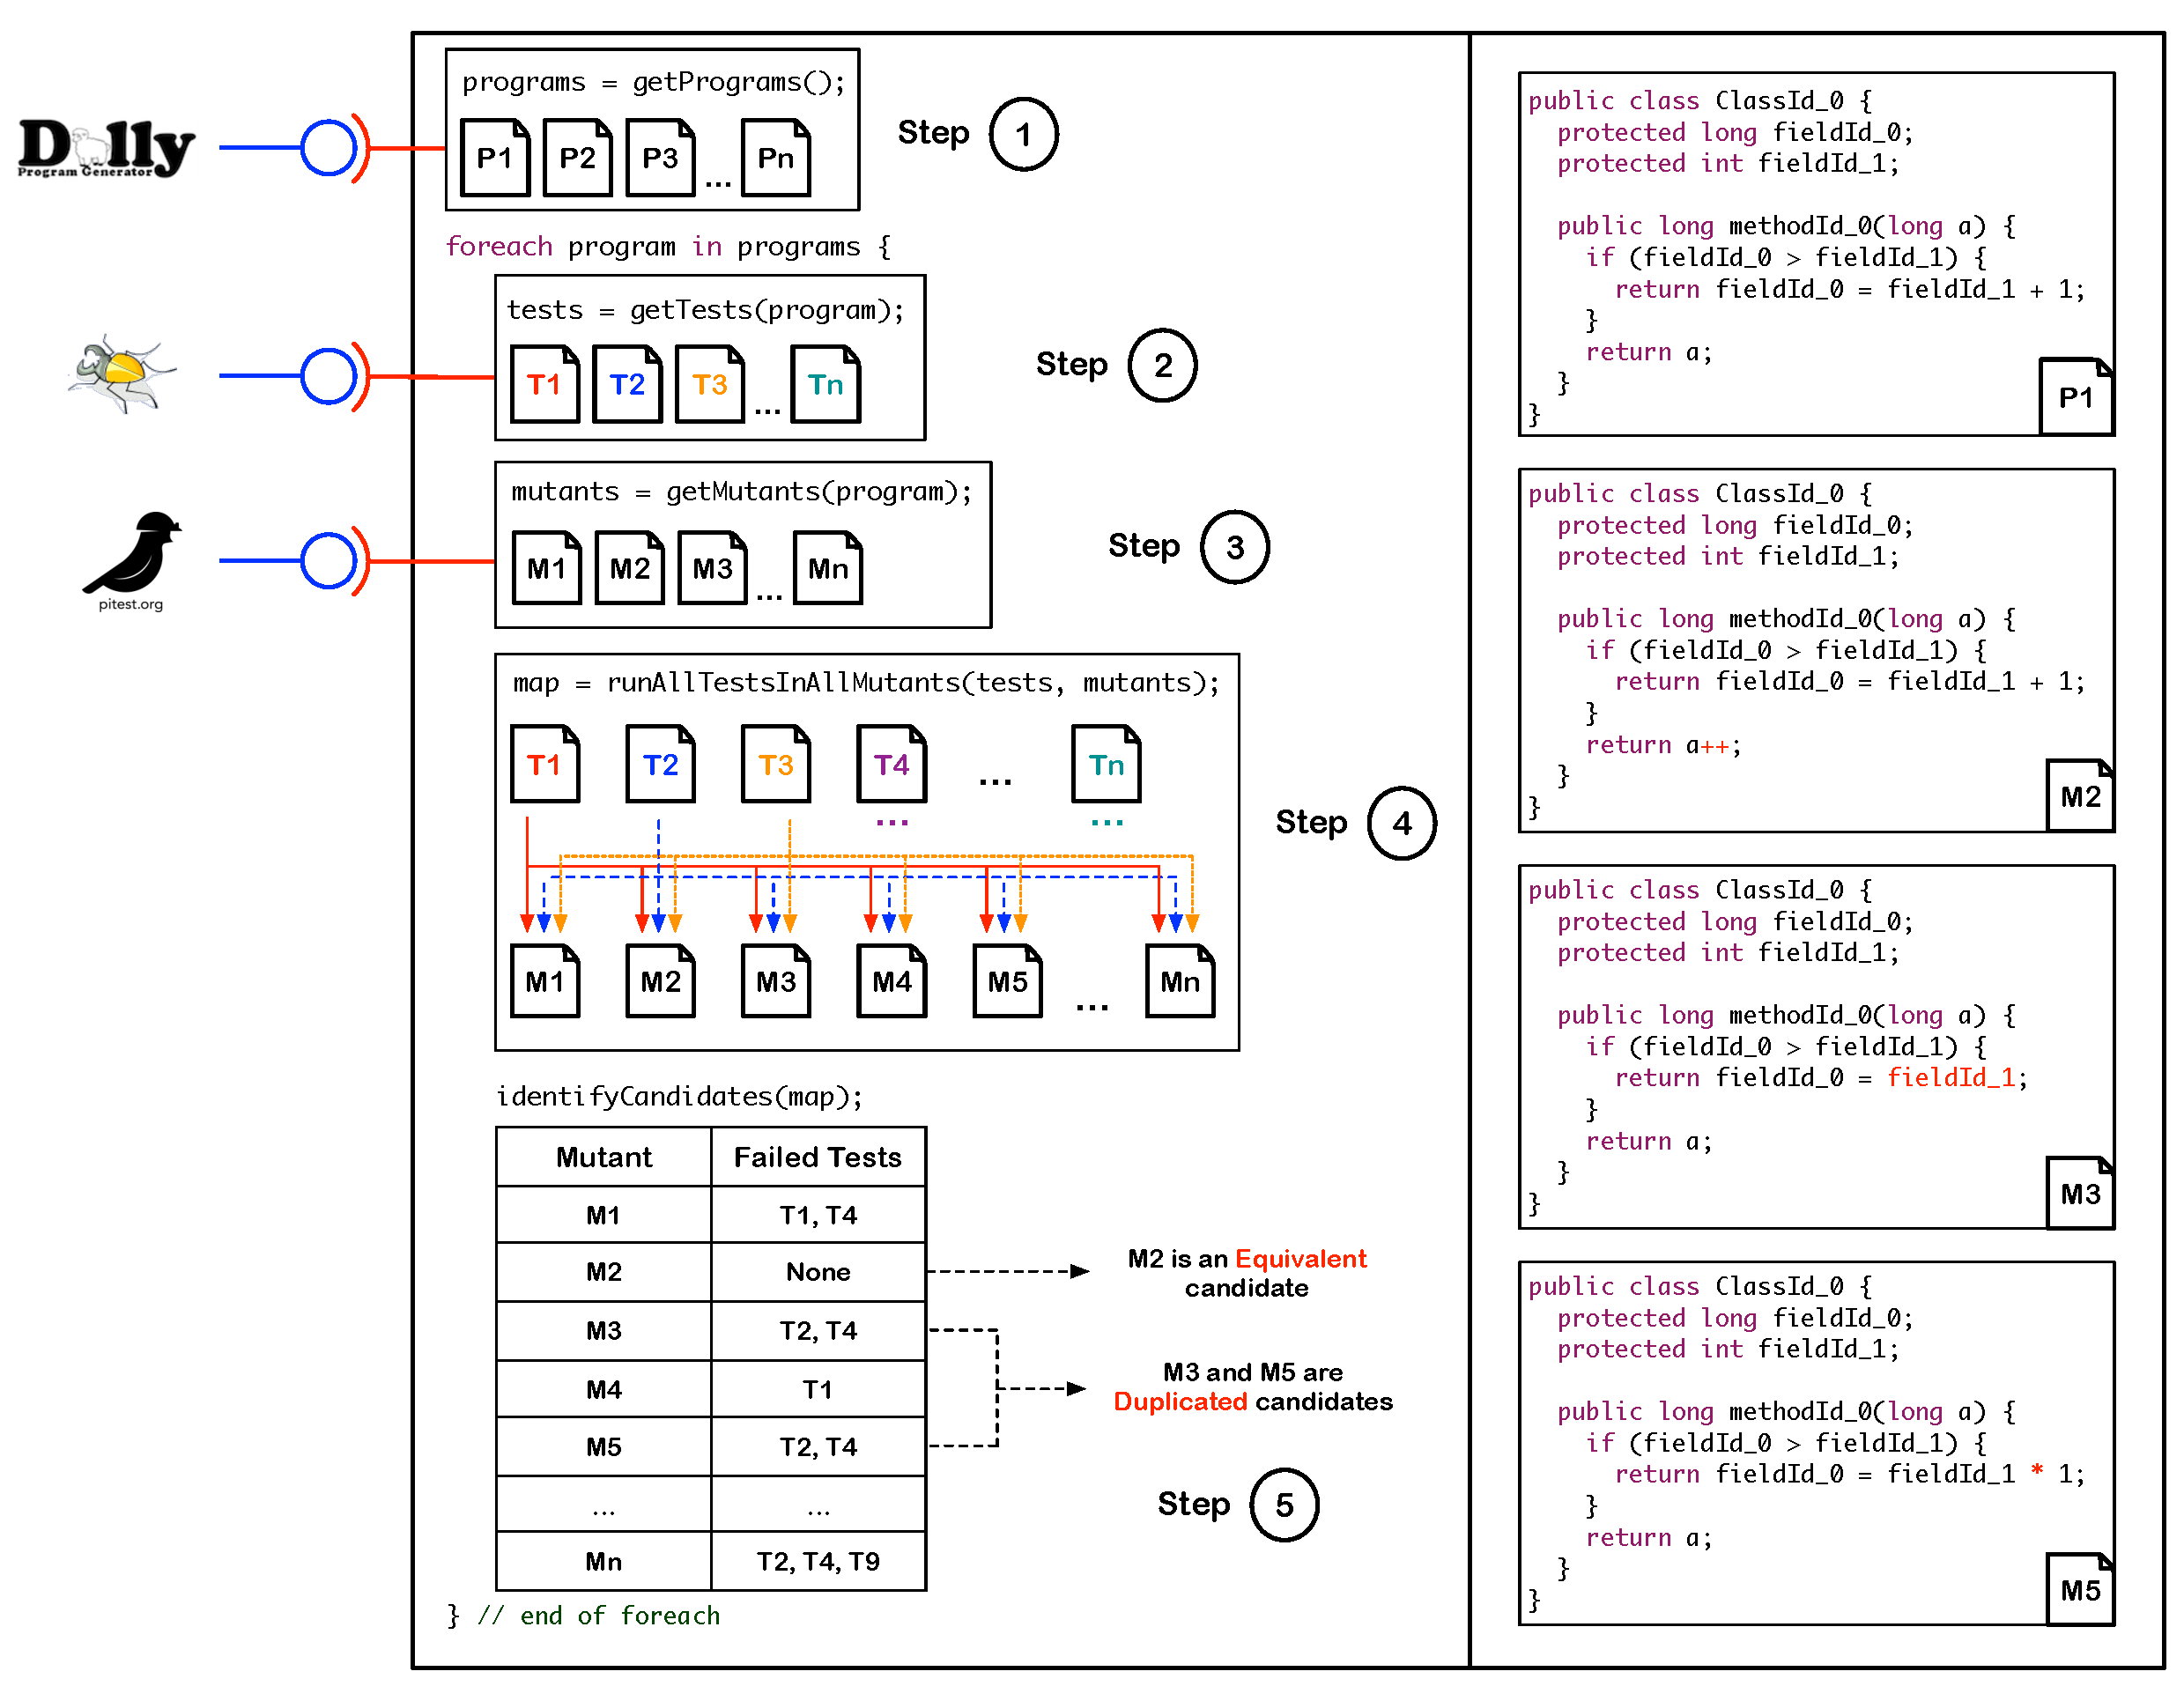
\includegraphics[scale=0.35]{images/Strategy.pdf}
		\caption{Strategy to identify equivalent and duplicated mutants candidates.}
		\label{fig:strategy}
	\end{center}
\end{figure*}


\section{Evaluation}
\label{sec:strategy-evaluation}

In this section, we execute our strategy to identify useless mutants candidates. 
By analyzing these candidates, we derive rules to avoid their generation (see Chapter~\ref{sec:rules}). 
We present the settings of our execution and then we discuss the results.

\subsection{Settings}

We intend to answer the following research question: \textit{Is the strategy capable of identifying useless mutants candidates?} 
To answer this question, we instantiate our strategy with \jdolly{}~\cite{SOARES:2013:1} to generate the set of programs; \randoop{} \cite{PACHECO:2007:1} as our test suite generator; and \mujava{}~\cite{OFFUTT:2005:1, OFFUT:2006:1}, \major{}~\cite{JUST:2011:1}, and \pit{}~\cite{PIT:2017} as our mutants generators.

\jdolly{} is an automated and bounded-exhaustive Java program generator based on Alloy, a formal specification language~\cite{alloy-book}. 
\jdolly{} receives as input an Alloy meta-model, which comprises a subset of possible Java constructs, and a scope, which is the maximum number of elements (classes, methods, fields, and packages) that the generated programs may declare, and optional constraints for guiding the program generation. 
It uses the Alloy Analyzer tool~\cite{alcoa}, which takes an Alloy specification and finds a finite set of all possible instances that satisfy the constraints within the specified scope. 
\jdolly{} then translates each instance found by the Alloy Analyzer to a Java program. 
It reuses the syntax tree available in Eclipse JDT for generating programs from those instances. 
Program \textit{P1} in Figure~\ref{fig:background} is a program generated by \jdolly{}. 

We execute our strategy to analyze \AnalyzedPrograms programs generated using \jdolly{}. 
In particular, we set \jdolly{} to generate programs with at most three fields (with or without overwriting), three methods (with or without overwriting and overloading), and two classes. 
One class always extends the other one. 
We also set \jdolly{} to use only the \texttt{int} and \texttt{long} primitive types. 
A class is the only non-primitive type. 
Moreover, each class is located into a package. 
If a class is not explicitly related to a package, the default package is assumed. 
Each field is associated with one identifier, one type, and at most one modifier, which can be protected or private. 
A method declaration contains a return type, an identifier, a parameter, a body, and a modifier related to its accessibility, which can be protected or public.

Since we use small and artificially-generated programs with no test suite, we  use \randoop{} as our test suite generator.
\randoop{}\footnote{\randoop{} stands for ``random tester for object-oriented programs''.}~\cite{PACHECO:2007:1} is an automatic unit test generator for Java. 
It generates unit tests, in JUnit format, using feedback-directed random test generation.
This means that it uses feedback obtained from executing a sequence of method calls and constructor invocation to create and mutate objects as it is being constructed. Then, it  uses this sequence of method calls plus an assertion about the result of a final method call to create the test.
Two types of tests are generated: error-revealing tests and regression tests. 
Error-revealing are tests that fail when executed, indicating a potential error in one or more classes under test.
Regression tests are tests that pass when executed and are useful in the future after a change in code.
%If the test passes right after its generation and it failures after a code change, then the change may have altered the program behavior.
\randoop{} is fully automatic, requires no input from the user (other than a class directory for Java) and, optionally, a time limit to generate tests. 
Previous experiments \cite{PACHECO:2007:1, PACHECO:2008:1} have shown that \randoop{} scales to realistic applications with hundreds of classes, which allowed it to find bugs in widely-deployed commercial and open-source software.

We acknowledge that the programs generated with \jdolly{} have a reduced scope when compared to industrial-scale systems and that random tests do not perform well for complex systems~\cite{ARTHO:2016:1} when compared with manually-made tests.
Nevertheless, previous work was capable of finding bugs in refactoring engines (e.g., Eclipse, JRRT, and NetBeans) by using a similar scope in \jdolly{} and with tests generated by \randoop{}~\cite{SOARES:2010:1, SOARES:2013:1, MONGIOVI:2014:1, MELINA:2017:1}.

%Given that our programs and the test set were built around the Java language, we search for Java mutation testing tools to generate the mutants.
%In the context of Software Engineering conferences, the three widely-used mutation testing tools for Java are \mujava{}, \pit{}, and \major{} \cite{KINTIS:2016:1}.
%So we chose those tools for our evaluation.

Regarding mutation testing tools, we selected \mujava{}, \pit{}, and \major{}.
These tools have different mutation operators.
In this evaluation, we use all available mutation operators of each tool (47 from \mujava{}, 9 from \major{}, and 13 from \pit{}).

%The next step of our strategy is to get all tests generated from each program and run against their respective mutants (Step~4). 
%The output of this is a table similar to that found in Figure \ref{fig:strategy} for each program.
%With this information, the strategy classifies the mutants as useful or useless (equivalent or duplicated) (Step~5).

%To check whether the mutants classified as useless are indeed useless, we manually analyze all of them together with the \AnalyzedPrograms programs.
It is important to note that we chose to use simple programs generated by \jdolly{}, instead of using complex Java programs, because it makes our entire evaluation feasible, since we wanted to explore all mutation operators from all mutation tools.
In addition, simple programs facilitate the manual analyses and minimize noise when reading and understanding the original and mutated programs.

\subsection{Results and Discussion}

We now present the results to answer our research question. 
As mentioned, we generated \AnalyzedPrograms programs based on \jdolly{}. 
The mutants generators yielded 4,999 mutants. 
Our strategy classified 963 mutants as equivalents and 1,332 mutants as duplicated. 
Table~\ref{tab:number-mutants} presents the results. 
Although we are using artificially generated programs, the numbers of equivalents and duplicated mutants are similar to the numbers presented in recent works~\cite{KINTIS:2017:1, KINTIS:2016:1}.

\scriptsize
\begin{table}[ht]
	\centering
	\caption{Useless mutants candidates identified.}
	\label{tab:number-mutants}
	\begin{tabular}{|l|c|c|c|}
		\hline
		& \textbf{Mutants} & \textbf{Equivalents}  & \textbf{Duplicated}    \\ \hline
		\mujava{} & 3,170    & 592 (18.6\%) & 1,089 (34.3\%) \\ \hline
		\major{}  & 816     & 166 (20.3\%) & 83 (10.1\%)   \\ \hline
		\pit{}    & 1,013    & 205 (20.2\%) & 160 (15.7\%)  \\ \hline
		TOTAL  & 4,999    & 963 (19.2\%) & 1,332 (26.6\%)  \\ \hline
	\end{tabular}
\end{table}
\normalsize

We detected some false positives, i.e., the strategy classified mutants as useless, but they are not. 
Table~\ref{tab:confusion-table} presents a confusion matrix to summarize our results. 
From 4,999 generated mutants (n), our strategy pointed 2,295 as useless and 2,704 as useful. 
Our manual analysis classified 204 out of 2,295 as false positives (FP) and 2,091 as true positives (TP). 
Notice that we did not have false negatives (FN) since our strategy found tests capable of killing all mutants pointed as useful. 
These numbers give us an accuracy of 95.92\%. 
When analyzing the false positives, we observed that some branches have not been covered by the test suite. 
It occurred because \randoop{} does not use techniques like symbolic execution~\cite{CORINA:2010:1}. 
This way, the generated tests could not kill any of the mutants that mutated code within such branches. 
This means that the quality of the test cases and their coverage play an important role in reducing false positives.

\scriptsize
\begin{table}[ht]
	\centering
	\caption{Confusion Matrix.}
	\label{tab:confusion-table}
	\begin{tabular}{|c|c|c|r|}
		\hline
		\multicolumn{2}{|c|}{\multirow{2}{*}{\textbf{n = 4,999}}} & \multicolumn{2}{c|}{\textbf{Actual}}                                 \\ \cline{3-4} 
		\multicolumn{2}{|c|}{}                                   & \textbf{true}                  & \multicolumn{1}{c|}{\textbf{false}} \\ \hline
		\multirow{2}{*}{\textbf{Predicted}}   & \textbf{true}    & \multicolumn{1}{r|}{2,091 (TP)} & 204 (FP)                            \\ \cline{2-4} 
		& \textbf{false}   & \multicolumn{1}{r|}{0 (FN)}    & 2,704 (TN)                           \\ \hline
	\end{tabular}
\end{table}
\normalsize

% We analyze the mutation operators more prone to generate useless mutants.
% Figure~\ref{fig:operators-equivalent} illustrates the number of equivalent mutants based on some mutation operators. 
% The AOIS operator (showed in Figure~\ref{fig:background}) was the one that generated the highest number of equivalent mutants. 
% This happens due to the several \texttt{return} statements generated by \jdolly{}. 
% Figure~\ref{fig:operators-duplicated} illustrates the number of duplicated mutants based on some mutation operators. 
% An example of two operators that together generated many useless mutants is COI (Conditional Operator Insertion) and ROR (Relational Operator Replacement).
% Given the following conditional expression \texttt{(x < y)}, COI generated \texttt{!(x < y)} whereas ROR generated \texttt{(x >= y)}. 
% So, one of these mutants is useless. 
% Given \texttt{(x == y)}, another example is COI generating \texttt{!(x == y)} and ROR generating \texttt{(x != y)}.

% \begin{figure*}[h]
% 	\begin{center}
		
% 		\subfigure[Equivalent mutants based on some mutation operators.] {
% 			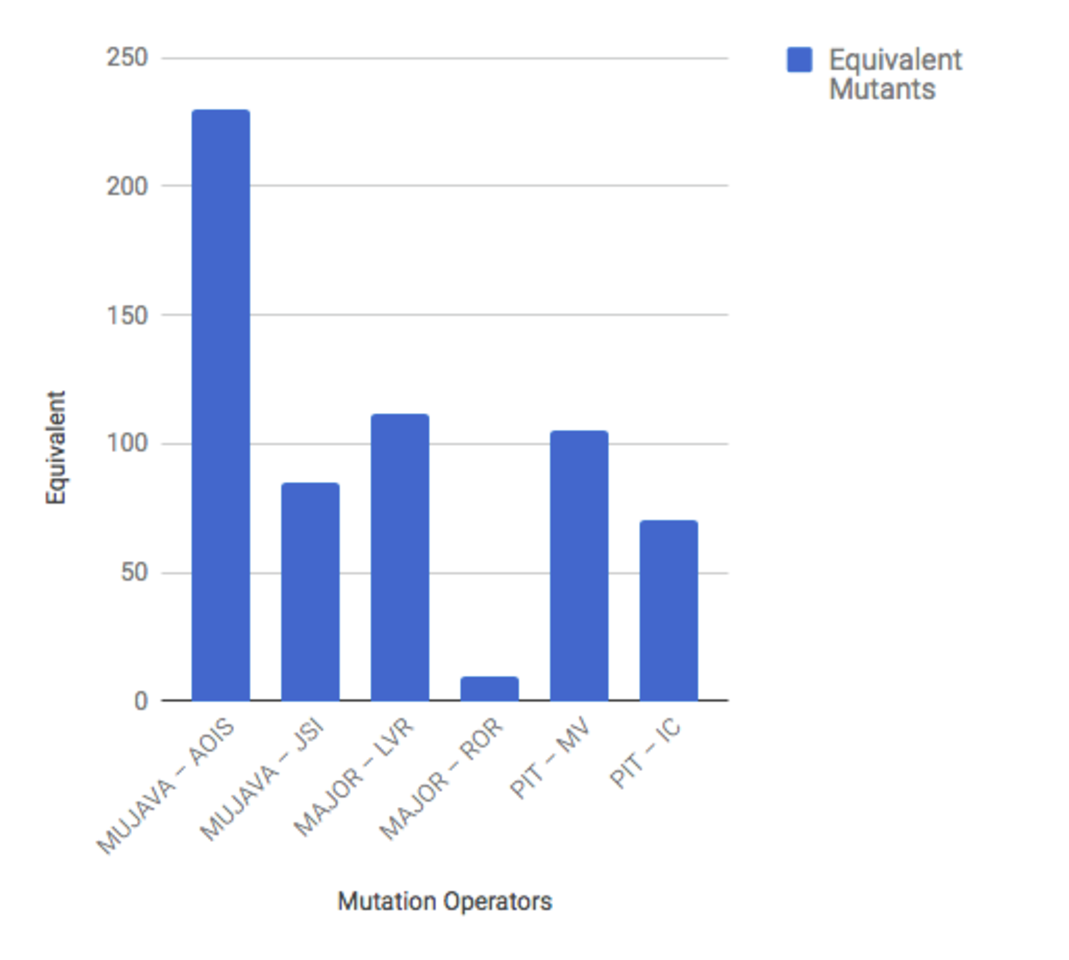
\includegraphics[scale=0.4]{images/EquivalentOperators.pdf}
% 			\label{fig:operators-equivalent}
% 		}
% 		\subfigure[Duplicated mutants based on some mutation operators.] {
% 			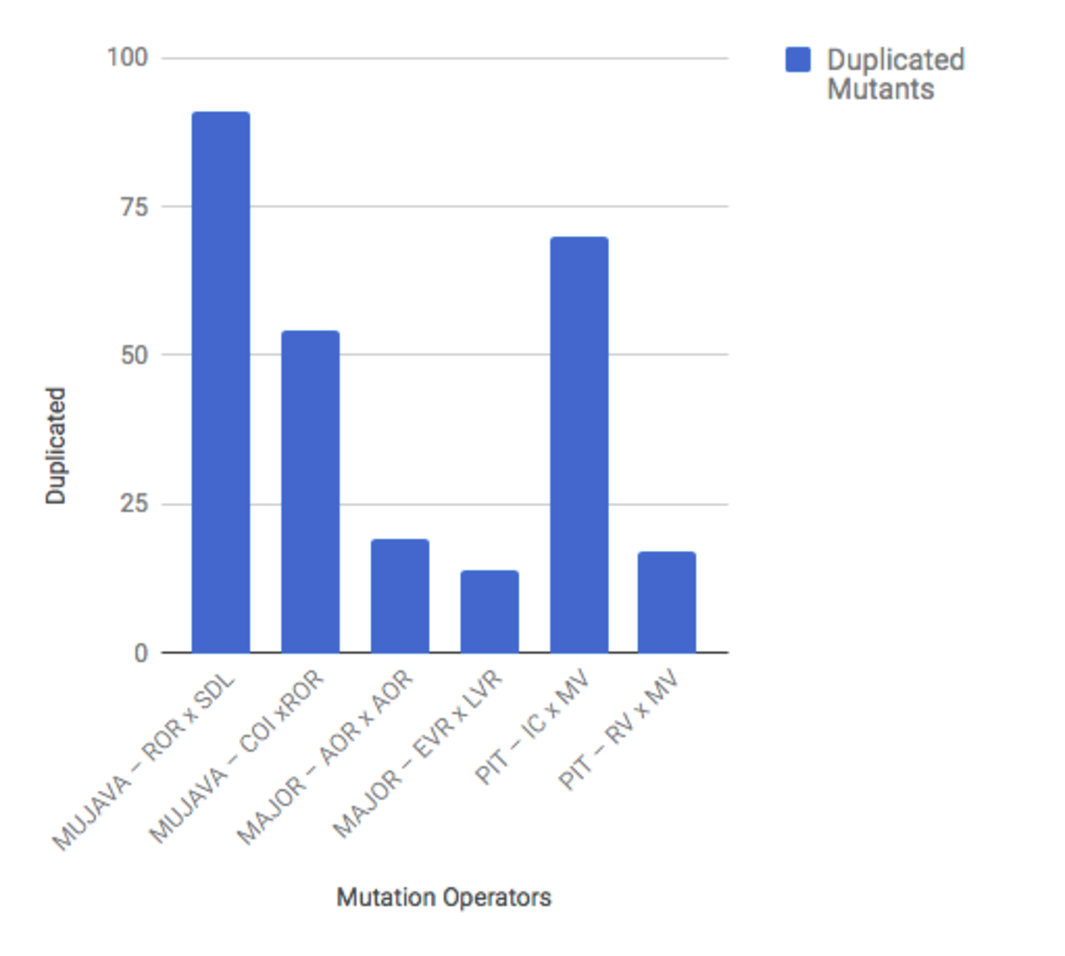
\includegraphics[scale=0.4]{images/DuplicatedOperators.pdf}
% 			\label{fig:operators-duplicated}
% 		}
		
% 		\caption{Equivalent and Duplicated mutants based on some mutation operators from the three mutation tools we used.}
		
% 	\end{center}
% \end{figure*}



This way, the answer to our research questions is yes, i.e., our strategy is capable of identifying useless mutants candidates. 
By using artificial and small Java programs, our strategy identified thousands of useless mutants with an accuracy of 95.92\% in our rating system.
%We do not know if our strategy would maintain the same performance using real programs, as we discuss in the Threats to Validity Section, but all this process is only the input to the real value of our work, that is deriving rules to avoid useless mutants.
Although the programs are simple, their mutants were crucial to derive those rules, as we shall see in Chapter~\ref{sec:rules}.


%\randoop{} did not generate a test to kill the mutants. For example, the JSI operator (Java Static Modifier Insertion) inserts the \texttt{static} keyword in class fields. In this case, \randoop{} could not generate a test to kill such mutants.

% \todo{
% For the mutants our strategy classified correctly as useless, but we could not derive rules, are the cases of coincidental correctness, that is, they are equivalent/duplicated, but at a very specific case we can not derive for a more general program.
% }

\subsection{Threats to Validity}
\label{sec:identifying-threats-to-validity}

The set of programs we used are based on a very few Java constructs. 
This is a threat to external validity. 
Still, this setup helped us to derive \NumberOfNewHeuristics new rules (Chapter~\ref{sec:rules}). 
In addition, the small programs allowed us to enable all available mutation operators from the three mutation tools we used in this work.

%Also, previous work could find bugs in refactoring engines (e.g., Eclipse, JRRT, and NetBeans) by using similar programs we used~\cite{SOARES:2010:1, SOARES:2013:1, MONGIOVI:2014:1, MELINA:2017:1}. 

Despite instantiating and executing the strategy only in Java programs, there is nothing particular to Java in our strategy. 
This means that it does not depend on the programming language. 
To use our strategy in other programming languages, all we need to do is to guarantee that everything is in the same language, i.e., programs, test suite, and mutants.

Our strategy identifies useless mutants candidates, which means it may lead to false positives. 
To weed out them, we rely on manual inspection, which is a threat. 
We minimized this threat by double checking all the useless candidates.

Another threat is that we set the \randoop{} time limit to three seconds. 
So, the tool has only three seconds to generate tests for a given program. 
In case we increase the time limit, we might reduce the number of false positives.

%\section{Introduction}
%\section{Better Discussion (RESULTS)}


\section{Research Status}
\label{sec:research-status-strategy}

We demonstrated that the strategy is capable of identifying useless mutants candidates.
However, we need to make some adjustments, add new features, and carry on the process improvement.

In what follows, we present the improvements we intend to perform.

\begin{enumerate}
    \item \textbf{Post-analysis: }We intend to add a \textit{post-analysis} in the final result of the strategy.
This post-analysis would try to extract information to facilitate the work of the programmer in deriving new rules.
For example, we could use a cluster algorithm to gather similar cases so as to indicate possible sites.
    \item \textbf{Execute the strategy with different instances: }We also intend to instantiate the strategy with different tools and setups.
For example, to derive more rules we intend to set our strategy to use different Java programs and different test suite generators (e.g., EvoSuite~\cite{FRASER:2011:1}).
    \item \textbf{Redundant Mutants: }Ammann et al.~\cite{AMMAN:2014:1} defines redundancy among mutants by identifying \textit{dominator mutants}, which subsume other mutants in the sense that mutant $m_i$ subsumes mutant $m_j$ if every test that kills $m_i$ also kills $m_j$. 
They demonstrated that a small set of mutants, approximately 1.2\%, subsumes all the others.
That is, approximately 99\% of all non-equivalent mutants are redundant.
%In \cite{PAPADAKIS:2016:1}, Papadakis et al. demonstrated that redundancy among mutants has a very good chance to inflate mutation score which puts in check all the studies that used such a metric.
\textit{Redundant mutants}, besides not adding anything to the mutation analysis, can inflate the mutation score \cite{PAPADAKIS:2016:1}, leading to misinterpretations about the outcome.
In summary, a small set of dominator mutants captures the power of the full set of mutants generated by a typical mutation system.
Redundant mutants could also be classified as useless.
As a next step we intend to adjust our strategy to classify redundant mutants candidates and extract rules to avoid them.
\end{enumerate}




%\subsection{Machine Learning}
%Machine learning allows a computer program to refine its decision-making abilities based on experience.

%Um outro passo que queremos discutir é a possibilidade de aliar técnicas de inteligência artificial a nossa estrategia, de maneira que a mesma possa aprender a derivar novas regras automaticamente, ou pelo menos dar fortes indicativos de descoberta de uma regra, a partir do que ela aprender olhando regras anteriores...








\chapter{Deriving Rules}
\label{sec:rules}

The identification of useless mutants is important to support developers on deriving rules to avoid the generation of such mutants. 
To derive the rules, we manually analyzed a total of 2,345 programs (50 programs + 963 equivalent mutants + 1,332 duplicated mutants). 
In this chapter, we first define what is a rule and then we illustrate several examples of rules we derived from the results of executing our strategy.


\section{Rule to Avoid Useless Mutants}
\label{sec:rules-definition}

To avoid the generation of these mutants, we develop rules.
A rule to avoid useless mutants is defined as a triple $(terms,~ transformations,~constraints)$, where:

\begin{itemize}
	
	\item \textit{term} is any Java language construct;
	
	\item \textit{transformations} is a set of mutation operators applied to \textit{term} or to one of its subterms; and
	
	\item \textit{constraints} is a set of conditions on $term$ or on the arguments of the mutation operators in $transformations$ that guarantee that the rule indeed avoids useless mutants.
	
\end{itemize}


In this context, \textit{term} represents the language constructs to which the \textit{transformations} (the mutations) will be applied. 
A rule to avoid an equivalent mutant (E-Rule) states that no mutation operator in \textit{transformation} should be applied whatsoever. 
On the other hand, a rule to avoid a duplicated mutant (D-Rule) states that only one of the mutation operators in \textit{transformations} should be applied. 
In this sense, by applying our rules right before the mutants generation, we can avoid useless mutants. 
To better explain the \textit{transformations} we use in our rules, we refer to the meta-variables presented in Table~\ref{tab:meta-variables}.

\scriptsize
\begin{table}[ht]
	\centering
	\caption{Meta-variables referred by the rules.}
	\label{tab:meta-variables}
	\begin{tabular}{|c|l|}
		\hline
		\textbf{Meta-variables} & \multicolumn{1}{c|}{\textbf{Description}} \\ \hline
		$op$         & any binary or unary operator \\ \hline
		$exp$        & any expression \\ \hline
		$b$          & any block of statements \\ \hline
		$s$          & any statement \\ \hline
		$;$          & an empty statement \\ \hline
		$C, D$          & class references \\ \hline
		$v$          & \begin{tabular}[c]{@{}l@{}}any identifier of variable, array access, or field \\ access for a primitive integral type (byte, short, int, long)\end{tabular} \\ \hline
	\end{tabular}
\end{table}
\normalsize

%Table~\ref{tab:mutationoperators} presents examples of \textit{transformations} performed by some mutation operators. 
%Notice that one operator may have more than one transformation, such as the ROR operator (Relational Operator Replacement).

Table~\ref{tab:mutationoperators} presents examples of \textit{transformations} performed by some mutation operators. 
For example, the LOI operator (Logical Operator Insertion) receives $v$ as input---see this meta-variable in Table~\ref{tab:meta-variables}---and returns $\sim v$. 
Mutation operators can also delete an entire statement. 
For instance, the SDL operator (Statement Deletion) deletes a given statement $s$, i.e., $SDL(s) =~;$~. 
The ROR operator (Relational Operator Replacement) has more than one transformation. 
The first and second transformations (ROR$_1$ and ROR$_2$) replace an entire expression by \texttt{false} and \texttt{true}, respectively. 
The third one (ROR$_3$) takes two binary operators as input, i.e., $op_1$ and $op_2$. 
Then, the operator replaces the first ($op_1$) by the second ($op_2$), as long as $op_1$ and $op_2$ $\in$ \{>, >=, <, <=, ==, !=\} and $op_1~\neq~op_2$.



%\scriptsize
\begin{table}[t]
	\centering
	\caption{Examples of transformations performed by some mutation operators. This table contains only a subset of all possible transformations performed by the mutation operators.}
	\label{tab:mutationoperators}
	\resizebox{\textwidth}{!}{%
	\begin{tabular}{|c|l|l|}
		\hline
		\textbf{Mutation Operators}                                                                        & \multicolumn{1}{c|}{\textbf{Transformations}}                                                                                                                                                                  & \multicolumn{1}{c|}{\textbf{Tool}} \\ \hline
		\begin{tabular}[c]{@{}c@{}}LOI \\ (Logical Operator Insertion)\end{tabular}                        & $LOI(v)~=~\sim~v$                                                                                                                                                                                           & \mujava{}                             \\ \hline
		\begin{tabular}[c]{@{}c@{}}LOD \\ (Logical Operator Deletion)\end{tabular}                         & $LOD(\sim~exp)$ = $exp$                                                                                                                                                                                           & \mujava{}                             \\ \hline
		\begin{tabular}[c]{@{}c@{}}ODL \\ (Operator Deletion)\end{tabular}                                 & \begin{tabular}[c]{@{}l@{}}$ODL_1(exp_1~op~exp_2) = exp_1$\\ $ODL_2(exp_1~op~exp_2) = exp_2$\end{tabular}                                                                                                                  & \mujava{}                             \\ \hline
		\begin{tabular}[c]{@{}c@{}}VDL \\ (Variable Deletion)\end{tabular}                                 & $VDL(v~op~exp) = exp$                                                                                                                                                                                            & \mujava{}                             \\ \hline
		\begin{tabular}[c]{@{}c@{}}AOIU \\ (Arithmetic Operator Insertion)\end{tabular}                                 & $AOIU(v) = -v$                                                                                                                                                                                            & \mujava{}                             \\ \hline
		\begin{tabular}[c]{@{}c@{}}AODU \\ (Arithmetic Operator Deletion)\end{tabular}                                 & $AODU(-exp) = exp$                                                                                                                                                                                            & \mujava{}                             \\ \hline
		\begin{tabular}[c]{@{}c@{}}ROR \\ (Relational Operator Replacement)\end{tabular}                   & \begin{tabular}[c]{@{}l@{}} $ROR_1(exp_1~op~exp_2) = false,~if~op~ \in~\{>,~>=,~<,~<=,~==,~!=\}$\\ 
			$ROR_2(exp_1~op~exp_2) = true,~if~op~ \in~\{>,~>=,~<,~<=,~==,~!=\}$\\ 
			$ROR_3(op_1,~op_2) = op_2,~if~op_1,~op_2~ \in~\{>,~>=,~<,~<=,~==,~!=\}~and~op_1~ \neq ~op_2$ \end{tabular} & \mujava{}                             \\ \hline
		\begin{tabular}[c]{@{}c@{}}SDL \\ (Statement Deletion)\end{tabular}                                & $SDL(s) =  $~$;$                                                                                                                                                                                                     & \mujava{}                             \\ \hline
		\begin{tabular}[c]{@{}c@{}}ISD \\ (super keyword deletion)\end{tabular}                            & $ISD(super.v) = v$                                                                                                                                                                                               & \mujava{}                             \\ \hline
		\begin{tabular}[c]{@{}c@{}}PNC \\ (new method call with child class type)\end{tabular}                            & $PNC(C, D) = D$                                                                                                                                                                                               & \mujava{}                             \\ \hline
		
		\begin{tabular}[c]{@{}c@{}}AOR \\ (Arithmetic Operator Replacement)\end{tabular}                   & $AOR(op_1,~op_2)~=~op_2, if~op_1,~op_2~\in~\{+,-,*,/,\%\}~$and$~op_1 \neq op_2$                                                                                                                                              & \major{}                              \\ \hline
		\begin{tabular}[c]{@{}c@{}}LVR \\ (Literal Value Replacement)\end{tabular}                         & \begin{tabular}[c]{@{}l@{}}$LVR(1) = 0$\\ $LVR(0) = 1$\end{tabular}                                                                                                                                                & \major{}                              \\ \hline
		\begin{tabular}[c]{@{}c@{}}InlineConstant \\ (Replaces inline constants)\end{tabular}               & \begin{tabular}[c]{@{}l@{}}$InlineConstant(1) = 0$\\ $InlineConstant(-1) = 1$\end{tabular}                                                                                                                         & \pit{}                                \\ \hline
		\begin{tabular}[c]{@{}c@{}}RemoveConditionals \\ (Replaces conditionals)\end{tabular} & $RemoveConditionals(exp) = false$                                                                                                                                                                  & \pit{}                                \\ \hline
		\end{tabular}
	}
\end{table}
%\normalsize

As an example, we now present a rule to detect an equivalent mutant. The ISD operator (super keyword deletion) deletes the \texttt{super} keyword from the $super.v$ term. In case $v$ exists only in the superclasses, the rule would prevent the mutation testing tool from applying the mutation operator in \textit{transformations}, i.e., the ISD operator, avoiding an equivalent mutant.
\\
\\
\textbf{E-Rule. ISD}\\
$term = super.v$\\
$transformations = \{\\ \indent ISD(super.v) =~v \\\}$\\
$constraints = \{ \\ \indent v$~exists~only~in~superclasses \\ $\}$\\

The aforementioned rule has been presented elsewhere~\cite{OFFUT:2006:1}. In the next section, we present a subset of the new rules we have identified.

\section{Examples of Rules}
\label{sec:examples-of-rules}

To better explain the rules we identified, we refer to six code snippets generated by our strategy presented in Figure~\ref{fig:useless-examples} (a--f). 
The left-hand side represents a code snippet from the original program. 
We underline the \textit{terms} to be transformed (mutated). 
To present examples of equivalents and duplicated mutants, we use two and three boxes, respectively. 
We present the mutation operators at the top of the boxes.

%\begin{figure*}[ht]
%	\begin{center}
%		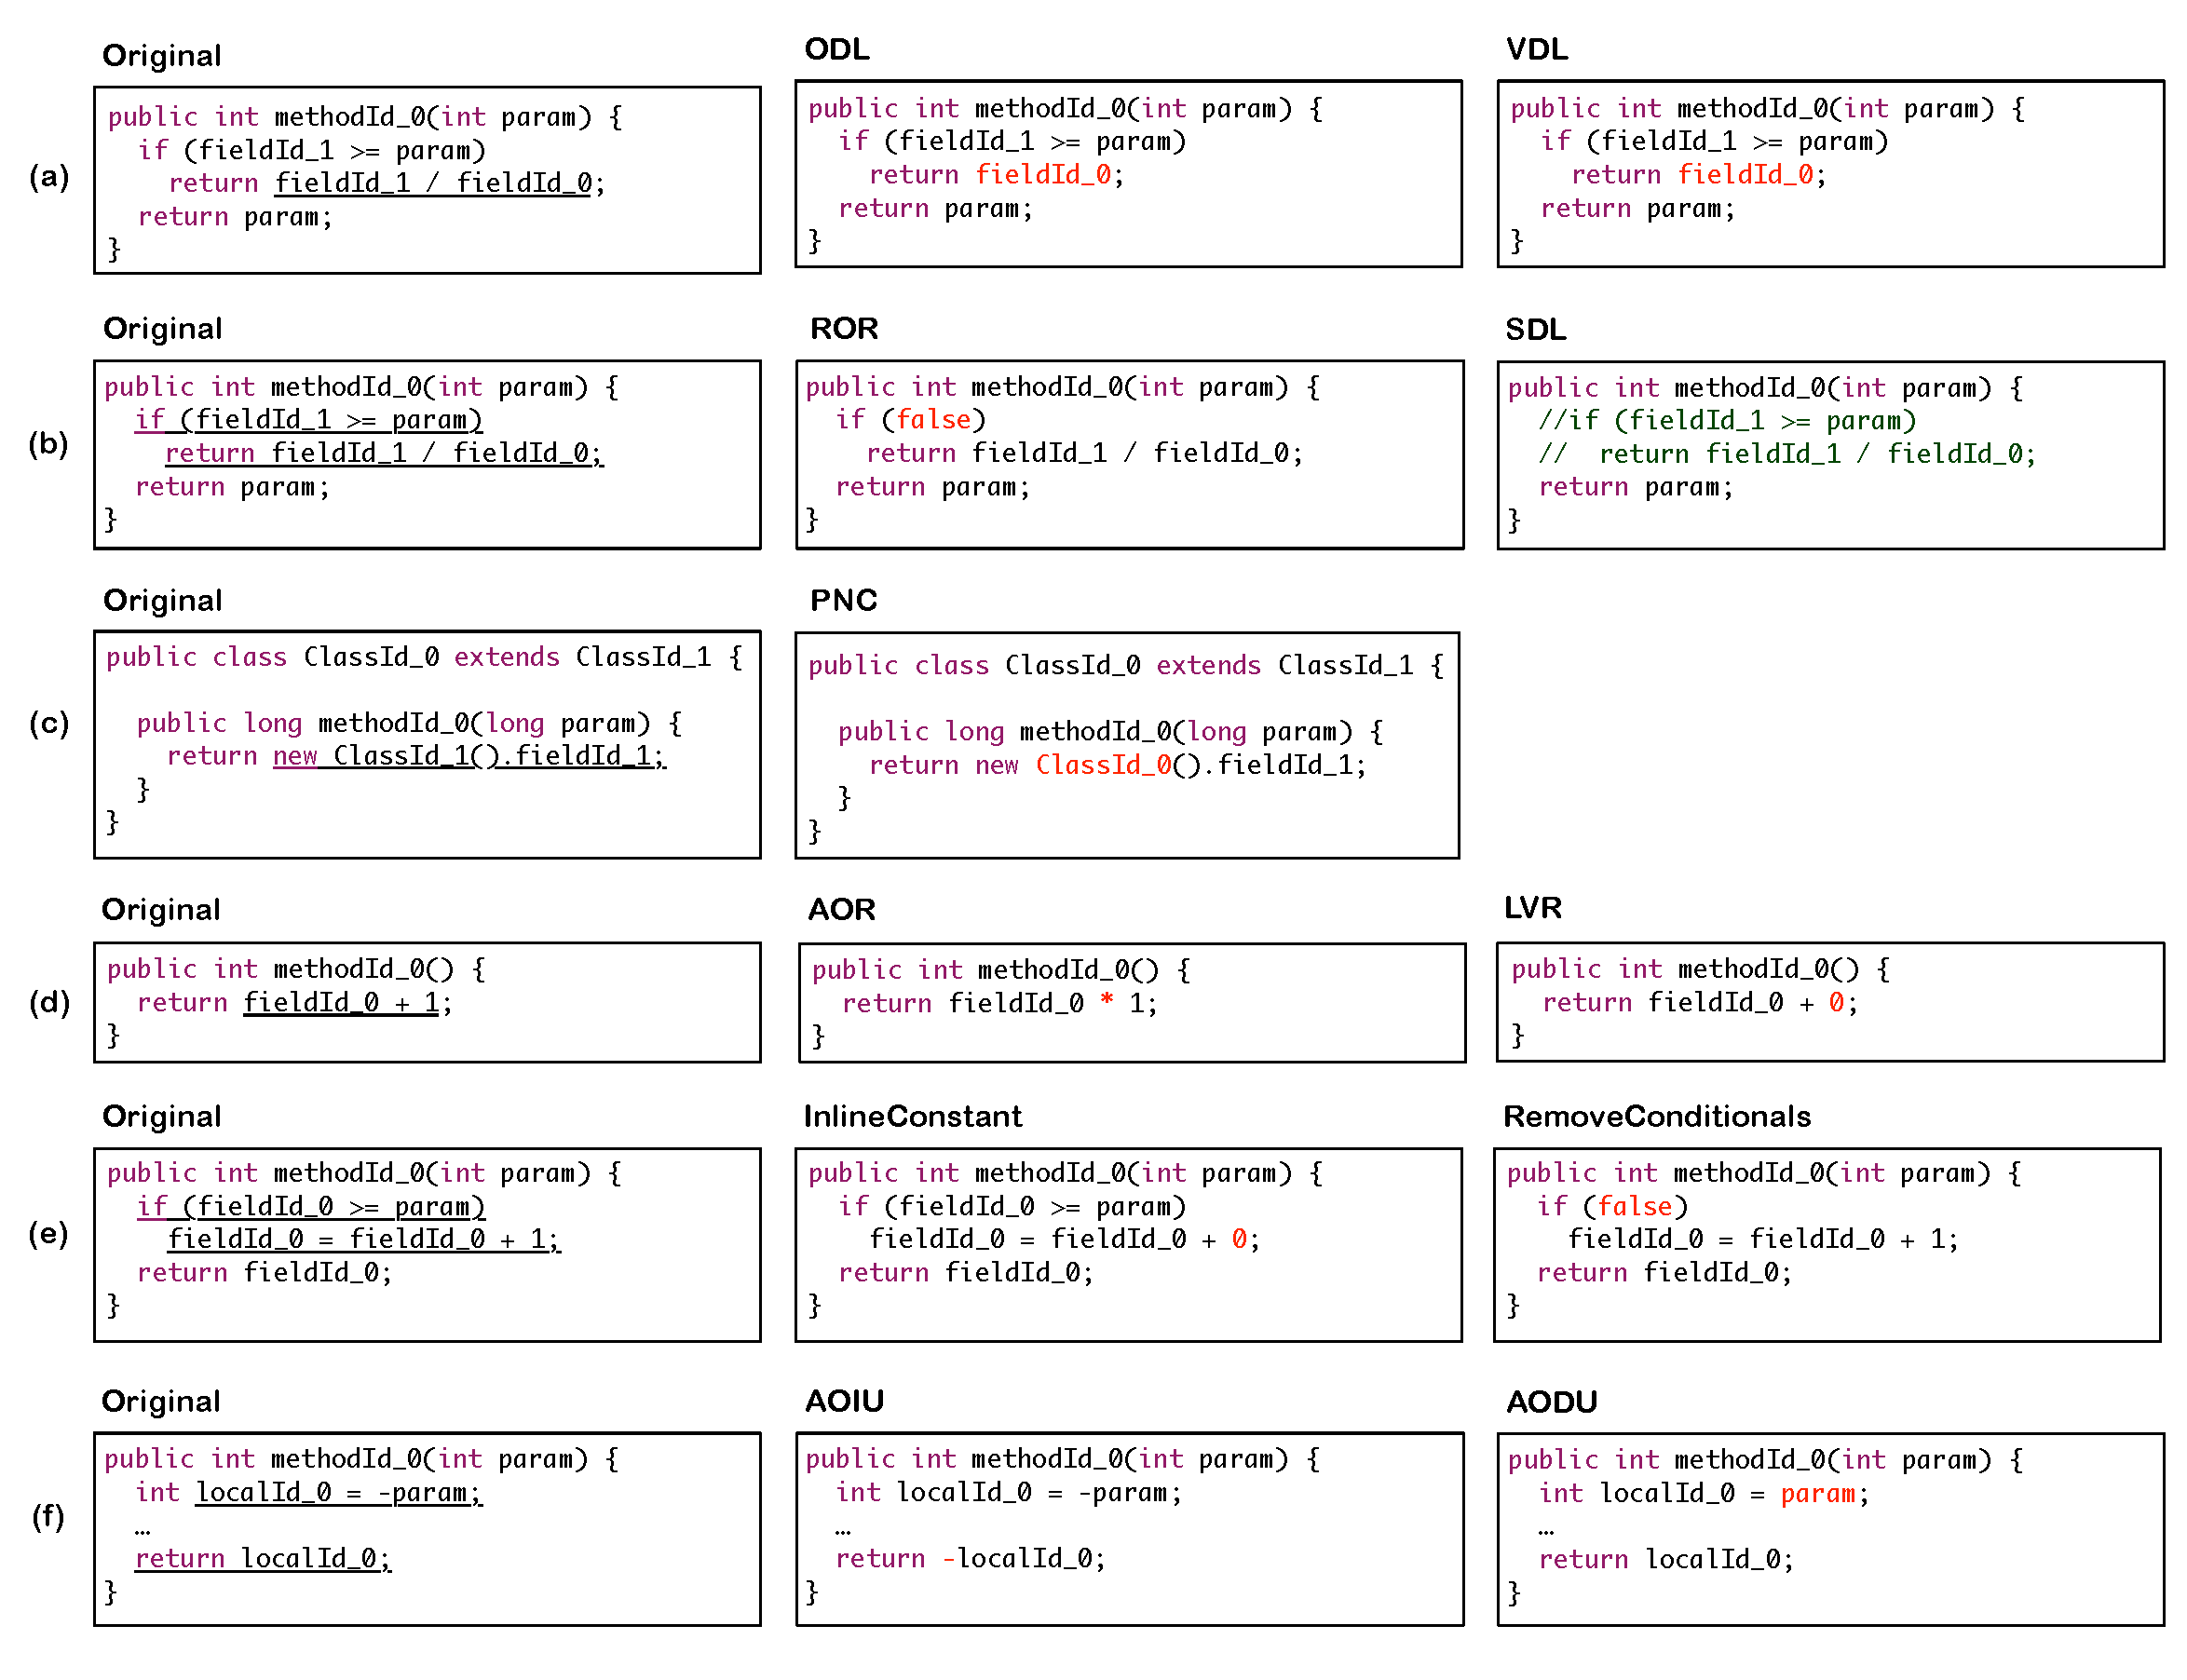
\includegraphics[scale=0.37]{images/Useless-Examples.pdf}
%		\caption{Original programs generated by \jdolly{} and useless mutants examples.}
%		\label{fig:useless-examples}
%	\end{center}
%\end{figure*}

\begin{figure*}[ht]
	\begin{center}
		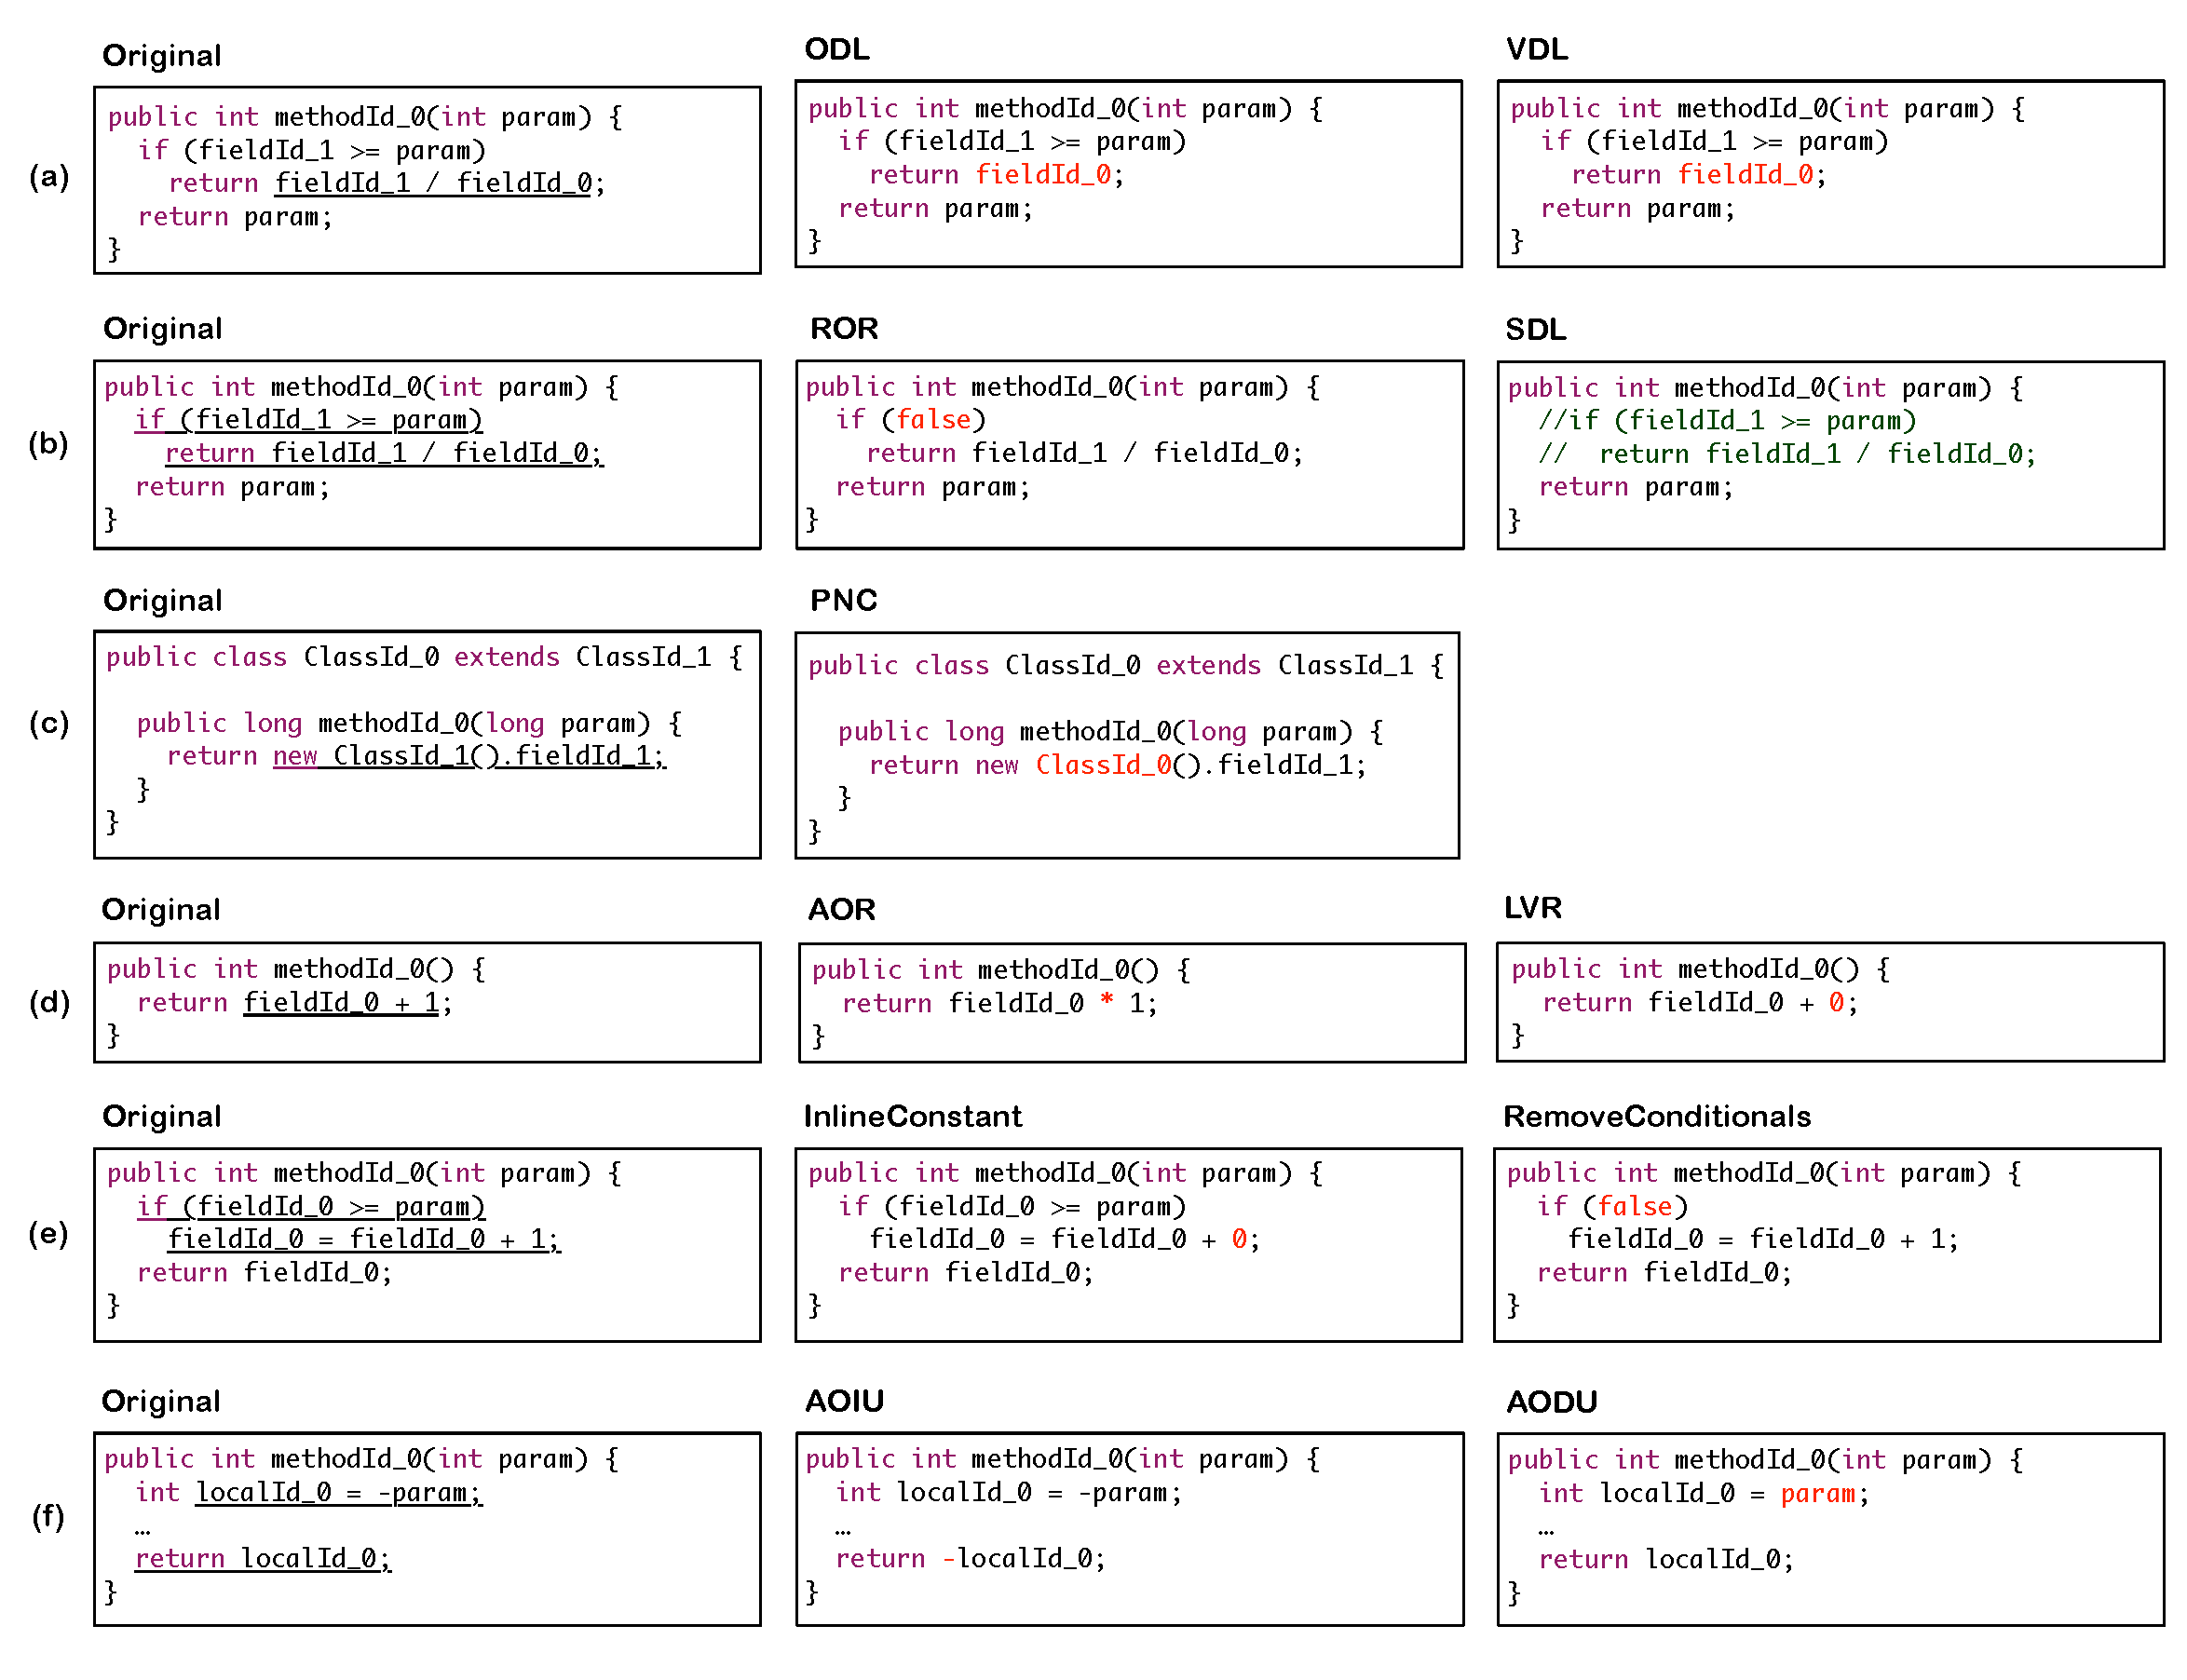
\includegraphics[scale=0.37]{images/Useless-Examples.pdf}
		\caption{Code snippets from programs generated by \jdolly{} and some of its useless mutants.}
		\label{fig:useless-examples}
	\end{center}
\end{figure*}

We now proceed as follows. Section~\ref{sec:no-def-use} presents rules that do not need \textit{def-use} analyses to be implemented. In contrast, Section~\ref{sec:def-use} presents rules that need \textit{def-use} analyses.

\subsection{Rules that do not need def-use analyses}
\label{sec:no-def-use}

Figure~\ref{fig:useless-examples}(a) illustrates an example of duplicated mutants with the exact same source code. These mutants have been generated by using the ODL and VDL operators (Operator and Variable Deletion). This way, according to the following rule, only one mutation operator in \textit{transformations} should be applied. The \textit{constraints} set is empty for this rule.
%We also identified a rule that can avoid the generation of mutants with the same exact source code. Figure~\ref{fig:useless-examples}(b) illustrates this case. The \mujava{} operators ODL and VDL (Operator and Variable Deletion) generated the same exact source code. This way, according to the following rule, only one mutation operator in \textit{transformations} should be applied. The \textit{constraints} set is empty for this rule.
\\
\\
\textbf{D-Rule. ODL x VDL}\\
$term = exp~op~v $\\
$transformations = \{\\ \indent ODL(exp~op~v) = exp,\\ \indent VDL(exp~op~v) = exp\\\}$\\

Figure~\ref{fig:useless-examples}(b) presents a code snippet that contains an \texttt{if} statement. Whilst the ROR operator (Relational Operator Replacement) sets the boolean expression to \texttt{false} (i.e., the \texttt{if} body will not be executed), the SDL operator (Statement Deletion) deletes the entire \texttt{if} statement. Therefore, these mutants are duplicated. We introduce a rule to identify this case as follows. Notice that the \textit{term} matches with an \texttt{if} statement without \texttt{else}. The \textit{constraints} set is empty.
%Figure~\ref{fig:useless-examples}(c) presents a program that contains an \texttt{if} statement. Whilst the ROR operator (Relational Operator Replacement) sets the boolean expression to \texttt{false} (i.e., the \texttt{if} body will not be executed), the SDL operator (Statement Deletion) deletes the entire \texttt{if} statement. Therefore, these mutants are duplicated. We introduce a rule to identify this case as follows. Notice that the \textit{term} matches with an \texttt{if} statement without \texttt{else}. The \textit{constraints} set is empty in this rule.
\\
\\
\textbf{D-Rule. ROR x SDL}\\
$term = if~(exp_1~op~exp_2)~\{b\} $\\
$transformations = \{\\ \indent ROR(exp_1~op~exp_2) = false, \\ \indent SDL(if~(exp_1~op~exp_2)~\{b\}) =~; \\ \}$\\

The next rule uses the bitwise complement operator ($\sim$), which simply flips bits (e.g., 00000010 becomes 11111101). To better explain this rule, consider that the original code contains a field with this operator (\texttt{$\sim$fieldId\_0}). In this context, when applying the \mujava{} operators LOI (Logical Operator Insertion) and LOD (Logical Operator Deletion) into the aforementioned field, we have duplicated mutants. In this example, LOI inserts the bitwise complement operator (\texttt{$\sim\sim$fieldId\_0}) and LOD removes (\texttt{fieldId\_0}). We define a rule to identify this case in what follows. In our rule, we apply LOI to the subterm $v$, not to the entire term $\sim$$v$. Notice that the \textit{constraints} set in this rule is empty.
%Figure~\ref{fig:useless-examples}(a) illustrates an example of duplicated mutants. Notice that the original code contains a field with a bitwise complement operator (\texttt{$\sim$fieldId\_0}). In this context, when applying the \mujava{} operators LOI (Logical Operator Insertion) and LOD (Logical Operator Deletion) into the aforementioned field, we have duplicated mutants (i.e., one of them is useless). In this example, LOI inserted the bitwise complement operator (\texttt{$\sim\sim$fieldId\_0}) and LOD removed (\texttt{fieldId\_0}). We define a rule to identify this case in what follows. In our rule, we apply LOI to the subterm $v$, not to the entire term $\sim$$v$. Notice that the \textit{constraints} set in this rule is empty.
\\
\\
\textbf{D-Rule. LOI x LOD}\\
$term = {\sim}v$\\
$transformations = \{\\ \indent LOI(v) = {\sim\sim} v,\\ \indent LOD({\sim}v) = v \\\}$\\

For the next rule, we avoid duplicated mutants that are generated by the same mutation operator. In the first mutant, the SDL operator (Statement Deletion) deletes the entire \texttt{if} statement; in the second one, it deletes the only statement within the \texttt{if} body. Notice that both mutants are duplicated, as long as \textit{constraints} hold: the \texttt{if} expression has no side effect. In this rule, \textit{term} matches with an \texttt{if} statement containing only one statement $s$ (refer to Table~\ref{tab:meta-variables}) without \texttt{else}.
%We also detected the same mutation operator generating duplicated mutants (see Figure~\ref{fig:useless-examples}(d)). In the first mutant, the SDL operator (Statement Deletion) deletes the entire \texttt{if} statement; in the second one, it deletes the only statement within the \texttt{if} body. Notice that both mutants are duplicated, as long as \textit{constraints} hold: the \texttt{if} expression has no side effect. In this rule, \textit{term} matches with an \texttt{if} statement containing only one statement $s$ (refer to Table~\ref{tab:meta-variables}) without \texttt{else}.
\\
\\
\textbf{D-Rule. SDL x SDL}\\
$term = if~(exp)~{~s~} $\\
$transformations = \{\\ \indent SDL(s) =~;, \\ \indent SDL(if~(exp)~s) =~; \\ \}$\\
$constraints = \{\\$ \indent $exp$~has~no~side~effect $\\\}$\\

%\todo{Esta regra nao necessita meso de def-use???}
We now present an E-Rule, i.e., a rule to identify equivalent mutants. We derived this rule by using a \mujava{} operator. Figure~\ref{fig:useless-examples}(c) shows a code example to better explain the rule. The PNC operator replaces superclass $C$ by subclass $D$. In this situation, field \texttt{v} must be declared only in $C$. In addition, the subclass constructor must not change \texttt{v} and calls the same superclass constructor defined in \textit{term}.
\\
\\
\textbf{E-Rule. PNC}\\
$term = new~C().v $\\
$transformations = \{ \\ \indent PNC(C, D)~=~D \\ \}$\\
$constraints = \{$ \\ \indent $D$~extends~$C$, \\ \indent $v$~exists only in$~C$, \\ \indent $D$~constructor does not change$~v$, \\ \indent $D$~constructor calls the same~$C$~constructor \\ \}$ $\\

The rules presented so far have been derived from mutation operators of \mujava{}. We now illustrate two rules derived by using \major{} and \pit{} operators. Figure~\ref{fig:useless-examples}(d) illustrates an example of duplicated mutants generated by \major{}. Notice that the original code contains the following binary expression: \texttt{fieldId\_0 + 1}. The AOR operator (Arithmetic Operator Replacement) replaces one operator by another. This way, AOR receives two operators as input in our rule, i.e., $op_1$ and $op_2$, and then replaces the first by the second. The LVR operator (Literal Value Replacement) replaces the literal one by the literal zero. In case we apply both mutation operators and \textit{constraints} hold, i.e., $op_1 \in \{+,-\}$ and $op_2 \in \{*,/\}$, we end up with duplicated mutants (e.g., \texttt{fieldId\_0 * 1} \textit{versus} \texttt{fieldId\_0 + 0}). We present a rule to avoid this situation in what follows.
\\
\\
\textbf{D-Rule. AOR x LVR}\\
$term =  exp~op_1~1 $\\
$transformations = \{ \\ \indent AOR(exp~op_1~1,~op_2) = exp~op_2~1, \\
\indent LVR(1)=0 \\ \}$\\
$constraints = \{\\ \indent op_1~\in~\{+, -\}~, \\ \indent op_2~\in~\{*, /\} \\ \}$\\

Now we present a rule we derived when using the \pit{} mutation testing tool. To better understand this rule, consider Figure~\ref{fig:useless-examples}(e). The InlineConstant operator replaced the literal one by the literal zero, yielding \texttt{fieldId\_0 = fieldId\_0 + 0;}. On the other hand, the RemoveConditionals operator changed the \texttt{if} expression to \texttt{false}. In this case, the first mutant does not change the \texttt{fieldId\_0} value. The second mutant does not change it as well, since the \texttt{if} body will not be executed. The rule to identify such case is presented in what follows. In this rule, notice that \textit{term} matches with an \texttt{if} statement containing only $v := v~op~1$ with no \texttt{else} statement.
\\
\\
\textbf{D-Rule. InlineConstant x RemoveConditionals}\\
$term = if~(exp)~{~v~:=~v~op~1} $\\
$transformations = \{ \\ \indent InlineConstant(1)~=~0,\\ \indent RemoveConditionals(exp)=false \\ \}$\\
$constraints = \{ \\$ \indent $op~\in~\{+, -\}$, \\ \indent $exp$~has~no~side~effect $ \\ \}$

\subsection{Rules that need def-use analyses}
\label{sec:def-use}

Using only the Abstract Syntax Tree (AST) is not enough to implement some of the rules we have identified. They need \textit{def-use} analyses. We now present a rule for this case. Whilst the AODU operator (Arithmetic Operator Deletion) removes the minus operator from the statement \texttt{localId\_0 = -param;}, the AOIU operator (Arithmetic Operator Insertion) inserts the minus at the \texttt{return} statement (\texttt{return -localId\_0;}). To better understand this rule, consider the code snippet presented in Figure~\ref{fig:useless-examples}(f). In this situation, one constraint does not allow us to implement this rule by using only the AST: there is neither a definition nor a use of the \texttt{localId\_0} variable in the block of code that lies between the assignment and the \texttt{return} statement.
\\
\\
\textbf{D-Rule. AODU x AOIU}\\
$term = v~:=~-exp;~b;~return~v$\\
$transformations = \{ \\ \indent AODU(-exp)~=~exp,\\ \indent AOIU(v)~=~-v \\ \}$\\
$constraints = \{ \\$ 
\indent there is no definition and use of $v$ in $b$, \\ 
\indent $v$ has local scope\\
\}\\
The next rule has the same \textit{constraints} of the previous one. In the first mutant, the LOI operator (Logical Operator Insertion) inserts the bitwise complement operator at the right-hand side of an assignment to a local variable \texttt{localId\_0}, i.e., \texttt{localId\_0 = $\sim$localId\_1}. In the second mutant, LOI inserts the bitwise into the \texttt{return} statement (i.e., \texttt{return $\sim$localId\_0;}). This situation yields duplicated mutants in case of constraints hold.
\\
\\
\textbf{D-Rule. LOI x LOI}\\
$term = v1 := v2; b; return~v1$\\
$transformations = \{\\ \indent LOI(v2) = {\sim} v2,\\ \indent LOI(v1) = {\sim} v1$\\\}\\
$constraints = \{\\$ 
\indent there is no definition and use of $v1$ in $b$, \\
\indent $v1$ has local scope \\
\}

\subsection{Summary}
\label{sec:rules-summary}

To the best of our knowledge, we have two new rules to avoid equivalent mutants and \NumberOfNewRulesForDuplicated new rules to avoid duplicated mutants. 
We have 25 rules derived from \mujava{} operators, 2 from \major{} operators, and 10 from \pit{} operators.
%\footnote{The complete set of rules can be found at the thesis' companion website: \url{https://sites.google.com/view/useless-mutants/}}

So far, we have presented nine rules. 
We now summarize the remaining 28 rules.\footnote{A detailed description of these rules can be found in Appendix A.} 
Seven rules involve infix arithmetic operators in their \textit{term}s: SDL x ODL, CDL x ODL, AORB x ODL, AORB x AORB, AOIS x CDL, InlineConstant x MemberVariable, and NonVoidMethodCall x InlineConstant. 
These mutation operators delete one side of arithmetic expressions or change the arithmetic operators. 
This situation may lead to useless mutants. 
For example, in case we have \texttt{v + 1}, ODL (Operator Deletion) and CDL (Constant Deletion) generates \texttt{v}. 
Another example is the application of the AORB (Arithmetic Operator Replacement) operator in two mutants, generating \texttt{v * 1} and \texttt{v / 1}.

Other seven rules are related to unary operators in their \textit{term}s, covering minus (\texttt{-}), bitwise complement (\texttt{$\sim$}), and logical complement (\texttt{!}). 
In case we have \texttt{v = -v;}, the ORU (Operator Replacement Unary) operator replaces \texttt{-} for \texttt{+}, and the STD (Statement Deletion) operator deletes the assignment statement. 
The following rules focus on similar cases: AODU x ODL, COD x ODL, LOD x ODL, ORU x STD, InlineConstant x Math, Math x MemberVariable, and InvertNegs x MemberVariable.

Five rules use the increment and decrement operators (SDL x VDL, ODL x AODS, AORS x ODL, AORS x LOI, and AORS x AOIU). 
For example, when having the statement \texttt{return ++v;}, in case \texttt{v} is local, the AORS (Arithmetic Operator Replacement) operator replaces the pre-increment for a post-increment and ODL (Operation Deletion) deletes the pre-increment operator.

Three rules involve relational operators in their \textit{term}s: COI x ROR, COD x ROR, and MemberVariable x RemoveConditional. 
In case we have the expression \texttt{v == 10}, we may have duplicated mutants. 
For example, COI (Conditional Operator Insertion) inserts the logical complement operator (\texttt{!}) before the expression, and ROR (Relational Operator Replacement) replaces  \texttt{==} for \texttt{!=}.

Five rules need \textit{def-use} analyses (ODL x LOI, IOD x ISI, ReturnVals x NonVoidMethodCall, InlineConstant x ReturnVals, and MemberVariable x ReturnVals). 
These rules use mutation operators that transform different parts of the code and their \textit{constraints} require that there is neither a definition nor a use of a variable in a block of code that lies between the two mutated statements.

All the cases above report D-Rules. We also introduce two E-Rules. We presented one of them in Section \ref{sec:examples-of-rules}. The other involves the JSI (Static Modifier Insertion) operator, which inserts the \texttt{static} keyword before each field declaration. In case the field is read-only, applying JSI is useless.

One might wonder that the terms and constraints presented in our rules are not common in practice, which means that the rules will not be often applied. To check whether the terms and respective constraints are common, we coun\-ted their occurrences in some well-known open-source systems. Table~\ref{tab:terms-in-common-systems} illustrates the occurrences of some terms and constraints we presented in this section. 
Notice that, in case we select the mutation operators used in this section, our rules have the potential to avoid thousands of useless mutants in each project.
Some rules are not so common. 
We have identified only four locations where the E-Rule PNC (column $new~C().v$ in Table~\ref{tab:terms-in-common-systems}) would apply.
In this case, the developer may choose to not implement it and avoid the extra analysis.

\scriptsize
\begin{table*}[t]
	\centering
	\caption{Occurrences of the terms we used in our rules in well-known open-source systems.}
	\label{tab:terms-in-common-systems}
	\resizebox{\textwidth}{!}{%
	\begin{tabular}{|l|c|c|c|c|c|c|c|c|c|c|}
		\hline
		\multicolumn{1}{|c|}{\textbf{Projects}} & \textbf{N. classes} & \textbf{$super.v$} & \textbf{${\sim}v$} & \textbf{$exp~op~v$} & \textbf{$if~(exp_1~op~exp_2)$} & \textbf{$if~(exp)~s$} & \textbf{$exp~op_1~1$} & \textbf{$if~(exp)~v~:=~v~op_1$} & \textbf{$new~C().v$} & \textbf{TOTAL} \\ \hline
		deeplearning4j                                  & 1,510                       & 17               & 28              & 1,161              & 3,103                      & 2,547                & 715               & 21                          & 2                & 9,104          \\ \hline
		eclipse.jdt.core                        & 2,001                       & 4                & 541              & 3,057              & 18,376                      & 15,780               & 3,993               & 195                          & 0                & 41,946          \\ \hline
		eclipse.platform.ui                     & 5,316                       & 50               & 58               & 1,791              & 15,561                      & 12,721               & 1,166               & 99                           & 0                & 31,446          \\ \hline
		j2objc                                  & 3,267                       & 88               & 138              & 2,693              & 11,285                      & 9,304                & 2,393               & 142                          & 0                & 26,043          \\ \hline
		kotlin                                  & 2,010                       & 5                & 674              & 165               & 4,410                       & 4,358                & 244                & 27                           & 0                & 9,883           \\ \hline
		neo4j                                  & 5,123                       & 4               & 38              & 666              & 3,469                      & 2,956                & 556               & 28                          & 1                & 7,718          \\ \hline
		spring-framework                        & 4,311                       & 9                & 5                & 372               & 5,544                       & 4,838                & 566                & 69                           & 0                & 11,403          \\ \hline
		wala                                  & 2,691                       & 27               & 12              & 551              & 4,198                      & 3,804                & 870               & 65                          & 1                & 9,528          \\ \hline
	\end{tabular}
}
\end{table*}
\normalsize

%Besides the ISD rule presented in Section~\ref{sec:rules-definition}, we also identified other rules already known by the mutation testing community. One example is a mutant that removes the initialization of a field initialized with its default value~\cite{PIT:2017}. Notice that, in case we do not initialize fields, Java does the job by initializing them with their default values. Thus, a mutant that removes such initialization is useless.


%-------------------------------------

In summary, we identified \NumberOfIdentifiedHeuristics rules. 
To the best of our knowledge, \NumberOfNewHeuristics out of \NumberOfIdentifiedHeuristics are new rules. 
We selected \mujava{} to implement our rules (Chapter~\ref{sec:implementing}) because we derived more rules by using this tool. In addition, when compared to \major{} and \pit{}, \mujava{} achieved the best results on simulating real practice bugs~\cite{KINTIS:2016:1}, but it was considered the most costly tool.
Therefore, solutions that lower their cost without losing their effectiveness can help the community.

\section{Research Status}
%Avoiding useless mutants using a lightweight approach is the best scenario to overcome the equivalent and duplicated mutant problems.
%To achieve this we define rules. 
%In the next chapter, we will show that it is enough to implement in a mutation tool.
%However, improvements need to be made in this part of the research.
%The following are the next steps we intend to take.
We intend to extend the work reported in this chapter in the following way:

\begin{enumerate}
    \item \textbf{Def-Use and other program analysis:}~We introduce some rules that need def-use analysis. In a previous work, Kintis and Malevris~\cite{KINTIS:2015:1} showed that a large portion of equivalent mutants can be avoided by just analyzing data-flow patterns in the original program under test. They implemented a tool called MEDIC. The tool uses the Static Single Assignment (SSA) \cite{ALPERN:1988:1} form of the original program to perform its analysis. MEDIC relies on T. J. Watson Libraries for Analysis (WALA) \cite{WALA:2017} framework to obtain such a representation. At the end, they propose a set of problematic data-flow patterns that tend to yields equivalent mutants. We plan to extend this tool to the idea of rules and thus prevent more useless mutants from being generated. In addition, we will calculate the trade-off of using a static program analysis tool in the mutation testing process.
    \item \textbf{Better Formalization:}~A rule is defined as a triple $(terms$, $ transformations$, $ constraints)$. We use a mixture of mathematical notation with a textual description. We believe that a better formalization of these rules may facilitate their understanding. So we intend to change this notation to something closer to a formal notation.
\end{enumerate}


%\subsection{More (new) Rules}
%\todo{...}




 


%For example, it could verify that apply AOIS at \textit{return fieldId\_0++} is not possible because it will yield an invalid statement, on the other hand apply AOIS at \textit{return a} will yield a valid mutant, which can being seen in mutant M2. However, in spite of valid, the mutant is useless, because it does not change the behaviour of the original program, so it is equivalent.

%Another example occurs when the user select the mutation operators XXX and YYY. A code location candidate to apply both operators are the statement ZZZZ. The mutation tool verify some conditions and allow the transformations, creating the mutants M3 and M5. However, the behaviour of both mutants are equivalent to each other, even not equivalent to the original. All the tests that kill M3 also kill M5, so one of them is unnecessary, that is useless.




%\section{Introduction}
%...

%\section{More Rules From GPCE (Spreadsheet)}
%...

\chapter{Evaluating the Rules}
\label{sec:implementing}

As mentioned, we identified the majority of the rules by using the \mujava{} mutation testing tool. 
%Also, when compared to \major{} and \pit{}, \mujava{} achieves the best results on simulating real bugs~\cite{KINTIS:2016:1}. 
So, we selected this tool to implement our rules. 
\mujava{} already has a small number of rules. 
In this way, to implement our rules, we followed the way \mujava{} developers implemented theirs. 
In addition, we used the same libraries to navigate through the Abstract Syntax Tree (AST) of a given program. 
We have implemented \NumberOfImplementedHeuristics rules that do not need \textit{def-use} analyses.

To check the potential of our rules, in this section we compute the number of useless mutants that our new \mujava{} version can prevent. 
By ``prevent'' we mean we \textit{do not generate} these mutants, reducing effort to generate, compile, and execute the test suite against such mutants.
To perform this computation, we execute the tool in industrial-scale systems.
Next, we first introduce how we implement the rules on \mujava{}, then
we present the evaluation of our rules.

\section{Rules on \mujava{}}
To implement the rules in \mujava{}, we decided to follow the same structure defined by the developers of the tool.
Each rule has a separate class file and extends a common class.
%This class acts like a \textit{visitor}.
%Then, at the moment right before generating the mutant, this class is called to evaluate the $term$, $transformations$, and $constraints$ of the rule.

Figure \ref{lst:code01} shows a code snippet of the rule AORB x AORB.
As explained in Section \ref{sec:rules-summary}, in case the user selects the mutation operator AORB and the $term$ refers to the binary expression \texttt{v + 1}, then four mutants are generated: \texttt{v * 1}, \texttt{v - 1}, \texttt{v / 1}, and \texttt{v \% 1}.
Two of them (\texttt{v * 1} and \texttt{v / 1}) are equivalents to each other.
So, only one of them is really useful.

To avoid these useless mutants we use conditional structures of the language.
The \texttt{isDuplicated} method (line 3-14 in Figure \ref{lst:code01}) receives the original expression and the mutated expression as parameter.
At line 5, the code verifies if the operator in the original binary expression is a \textit{plus} or \textit{minus}. 
Then, at line 7, the code verifies if the right-hand side of the binary expression is the literal \textit{one}.
For this rule, the final verification (line 8) discards the mutant if the mutated code has the \textit{division} operator.
%In this case, as can be seen in Figure \ref{lst:code01}, we decided to discard~ \texttt{v / 1}.

\begin{figure}[thp] % the figure provides the caption
\centering          % which should be centered
\caption{Code snippet of a rule on \mujava{}}
\begin{tabular}{c}  % the tabular makes the listing as small as possible and centers it
\begin{lstlisting}[label={lst:code01}, basicstyle=\fontsize{7.5}{11}\ttfamily, linewidth=.95\linewidth]
public class AORB_x_AORB extends DRule {
    ...
    private boolean isDuplicated(BinaryExpression original, BinaryExpression mutant) {
        int op = original.getOperator();
        if (op == BinaryExpression.PLUS || op == BinaryExpression.MINUS) {
            Expression right = original.getRight();
            if (right instanceof Literal && ((Literal)right).equals(Literal.constantOne())) {
                if (mutant.getOperator() == BinaryExpression.DIVIDE) {
                    return true;
                }
            }
        }
        return false;
    }
}
\end{lstlisting}
\end{tabular}
\end{figure}

All classes that extend \texttt{DRule} have access to all the mutation operators selected by the user, so we only apply a D-Rule if the operators involved are selected.

An E-Rule has a similar approach, however, it does not need to know the mutation operators selected by the user.

In the rest of the chapter we will show how we evaluate the rules implemented in \mujava{}.


\section{Evaluation}
\label{sec:evaluation}
In this section, we detail how we performed the execution of our new \mujava{} version embedded with the rules.
We start by showing the settings and we end up discussing the results. 
Last but not least, we present the threats to validity.

\subsection{Settings}
\label{sec:evaluation-settings}

We intend to answer the following research questions: 

\begin{itemize}
    
    \item \textit{Are the rules capable of avoiding useless mutants in industrial-scale systems?}
    
    \item \textit{What is the overhead of executing our rules in industrial-scale systems?}

\end{itemize}

It is important to answer these questions because we derived our rules based on small and artificially generated programs. 
To answer the first question, we selected six open-source projects that vary in size and application domain. 
These projects have been used in previous mutation testing research~\cite{KINTIS:2017:1, PAPADAKIS:2015:1, JUST:2014:1, KINTIS:2015:1}. 
We list the projects in Table~\ref{tab:systems}. 
However, to make our analysis feasible, we follow the same procedure applied in~\cite{KINTIS:2017:1}. 
For each project, we rank all packages according to their size. 
Then, we select the three largest classes that could be handled without a problem by \mujava{}\footnote{\mujava{}~4 uses the OJ~1.1 (\url{https://www.csg.ci.i.u-tokyo.ac.jp/openjava/}) parser. 
This parser does not support some Java constructs, such as generics and for-each loops.} among the four largest packages. 
This way, we selected classes of different sizes. 
For example, for the \textit{h2} project, we have classes with 115 LOC, 253 LOC, 1,542 LOC, and 5,895 LOC. In this particular setup, we focus on 72 classes, 12 per project. 


\scriptsize
\begin{table}
    \caption{Open-source projects we used to execute the \mujava{} version enhanced with our rules.}
    \centering
    \begin{tabular}{|c|c|c|}
    \hline
    \textbf{System} & \textbf{Domain} & \textbf{LOC} \\
    \hline
    ant-1.8.4 & Build system & 104,479 \\
    \hline
    bcel-5.2 & Bytecode manipulation & 23,726 \\
    \hline
    commons-lang-2.4-src & Java core classes & 18,168 \\
    \hline
    commons-math-1.2-src & Math library & 16,753 \\
    \hline
    h2-1.0.79 & Database application & 72,359 \\
    \hline
    joda-time-2.4 & Date and time utility & 28,255 \\
    \hline
    \end{tabular}
    \label{tab:systems}
\end{table}
\normalsize

We then executed our new \mujava{} version. 
However, instead of discarding the useless mutants identified by our rules, we generated and labeled them. 
This is important to validate our rules implementation, confirming whether the labeled mutants are indeed useless or not.

To perform the validation of our rules, we have two steps. 
First, we submit the original classes and the useless mutants candidates to a sound tool, TCE (Trivial Compiler Equivalence), presented in recent research~\cite{KINTIS:2017:1}.
Given two java files (original \textit{versus} mutant or mutant \textit{versus} mutant), TCE applies compiler optimizations and check their bytecode. 
In case they are the same, TCE guarantees that the files are equivalent. 
This way, we consider that our rules are correct in case they labeled the useless mutants confirmed by TCE. 
In the second step, we list the ones not confirmed by TCE and manually analyze a subset of those mutants. 
For each class (out of 72), we randomly select 10\% of the useless mutants identified by each rule. 
To better explain this selection, suppose we have 100 useless mutants identified by four of our rules and not confirmed by TCE (50 by Rule~A, 30 by Rule~B, 10 by Rule~C, and 10 by Rule~D). 
In this situation, we randomly select 10\% of mutants identified per rule, i.e., 5 from Rule~A, 3 from Rule~B, 1 from Rule~C, and 1 from Rule~D. 
In this way, our manual analysis comprised all rules we implemented in \mujava{}.

To answer the second question, we compare the execution time of the original \mujava{} with our new \mujava{} version. 
The execution time encompasses the time to generate mutants and compile them. 
For this research question, we re-executed the entire experiment (three times and considered the average), but now our \mujava{} version discards the useless mutants, instead of generating and labeling them as useless. 
We use the same six open-source projects to compute the time.


\subsection{Results and Discussion}
\label{sec:evaluation-results}

In this section, we present the results and answer our research questions. 
Table~\ref{tab:real-practice-subjects} presents the results. 
%During the execution of our study, we disabled the few rules that \mujava{} already had. 
%This way, Table~\ref{tab:real-practice-subjects} presents only data with respect to our rules. 
We illustrate the number of mutants and the number of equivalents and duplicated mutants per project. 
For example, our rules detected 3,903 (10.94\%, i.e., 3,903/35,669) duplicated mutants in the \textit{h2} project. 
TCE confirmed 2,276 (58.31\%) duplicated mutants out of the 3,903 our rules identified. 
This way, we have 1,627 mutants of real classes to analyze. 
As mentioned, to make our manual analysis feasible, we randomly selected and analyzed 10\% of the useless mutants identified by each rule. 
In this manual task, we faced a few bugs in our rules implementation (e.g., one constraint missing). 
After fixing these bugs in our rules, we re-executed the entire analysis until we confirm all useless mutants pointed by our rules.
In the last execution, we did not identify false positives in the random subset we manually analyzed. 
This way, despite being derived from artificial and small Java programs, our rules could identify useless mutants in industrial-scale projects. 
On average, they identified almost \textbf{13\%} of useless mutants (i.e., \textbf{1.70\%} of equivalents and \textbf{11.13\%} of duplicated).


\scriptsize
\begin{table}[t]
\centering
\caption{Results of executing \mujava{} with our rules.}
\label{tab:real-practice-subjects}
\begin{tabular}{|l|c|l|r|r|r|c|}
\hline
\multicolumn{1}{|c|}{\textbf{Project}} & \textbf{Mutants}        & \multicolumn{1}{c|}{\textbf{}} & \multicolumn{1}{c|}{\textbf{\#}} & \multicolumn{1}{c|}{\textbf{\%}} & \multicolumn{2}{c|}{\textbf{Confirmed TCE}} \\ \hline
\multirow{2}{*}{ant}                   & \multirow{2}{*}{13,695}  & Eq.                    & 156                              & 1.14\%                           & 58                   & 37.18\%                 \\ \cline{3-7} 
                                       &                         & Dup.                     & 1,761                             & 12.86\%                          & 994                  & 56.45\%                 \\ \hline
\multirow{2}{*}{bcel}                  & \multirow{2}{*}{17,491}  & Eq.                    & 251                              & 1.44\%                           & 154                  & 61.35\%                 \\ \cline{3-7} 
                                       &                         & Dup.                     & 2,292                             & 13.10\%                          & 1,600                 & 69.81\%                 \\ \hline

\multirow{2}{*}{commons-lang}          & \multirow{2}{*}{33,878}  & Eq.                    & 900                              & 2.66\%                           & 710                  & 78.89\%                 \\ \cline{3-7} 
                                       &                         & Dup.                     & 4,049                             & 11.95\%                          & 2,831                 & 69.92\%                 \\ \hline
\multirow{2}{*}{commons-math}          & \multirow{2}{*}{21,737}  & Eq.                    & 212                              & 0.98\%                           & 131                  & 61.79\%                 \\ \cline{3-7} 
                                       &                         & Dup.                     & 1,903                             & 8.75\%                           & 1,427                 & 74.99\%                 \\ \hline
\multirow{2}{*}{h2}                    & \multirow{2}{*}{35,669}  & Eq.                    & 320                              & 0.90\%                           & 243                  & 75.94\%                 \\ \cline{3-7} 
                                       &                         & Dup.                     & 3,903                             & 10.94\%                          & 2,276                 & 58.31\%                 \\ \hline
\multirow{2}{*}{joda-time}             & \multirow{2}{*}{13,024}  & Eq.                    & 463                              & 3.55\%                           & 403                  & 87.04\%                 \\ \cline{3-7} 
                                       &                         & Dup.                     & 1,166                             & 8.95\%                           & 817                  & 70.07\%                 \\ \hline
\multirow{2}{*}{TOTAL}                 & \multirow{2}{*}{135,494} & Eq.                    & 2,302                             & 1.70\%                           & 1,699                 & 73.81\%                 \\ \cline{3-7} 
                                       &                         & Dup.                     & 15,074                            & 11.13\%                          & 9,945                 & 65.97\%                 \\ \hline
\end{tabular}
\end{table}
\normalsize

These results are quite encouraging. 
In a recent work~\cite{KINTIS:2017:1}, researchers summarized dozens of related work on useless mutants. 
Only a few provided techniques to \textit{avoid} their generation \cite{ADAMOPOULOS:2004:1, MADEYISKI:2014:1}. 
However, they focused only on equivalent mutants. 
In this work, we also provide rules to avoid duplicated mutants. 
Still, one might claim that the number of useless mutants avoided presented in Table~\ref{tab:real-practice-subjects} is low. 
Nevertheless, notice that we have implemented only \NumberOfImplementedHeuristics rules. 
In addition, we can derive more rules in case we use our strategy with more complex Java programs, contributing to increasing the number of avoided useless mutants.

We analyzed how often the rules were applied across all projects.
In Figure \ref{fig:rules-duplicated} we observe that five D-Rules accounted for approximately 87\% of the duplicated mutants avoided.
With emphasis on mutation operators: ODL (Operator Deletion), SDL (Statement Deletion), and ROR (Relational Operator Replacement). 
They appear in all five highlighted rules.
The D-Rule SDL x SDL avoided almost a quarter of all duplicated mutants identified by our rules.
This rule can be seen in the Section \ref{sec:no-def-use}.
This result shows that the analyzed systems have many conditional blocks with only one statement in their body and the \texttt{if} expression has no side effect.
The second most applied D-Rule was CDL x ODL.
It is similar to VDL x ODL (presented in Section \ref{sec:no-def-use}), with the difference that CDL is applied to code constants, while VDL is applied to code variables.
These mutation operators occur, frequently, in unary and binary Java expressions involving mathematical operators.
The D-Rule COI x ROR (explained in Section \ref{sec:rules-summary}) was the fourth most applied. 
This rule occurs in conditional expressions involving \texttt{==} or \texttt{!=}.
ROR x SDL was presented in Section \ref{sec:def-use}. 
It occurs in \texttt{if} statements that have relational operators in their conditional expression.

\begin{figure*}[htb]
	\begin{center}
		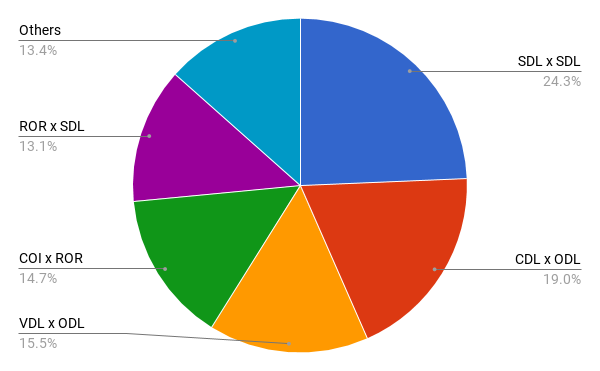
\includegraphics[scale=0.5]{images/chart-total-rules-duplicated.png}
		\caption{D-Rules that avoided more duplicated mutants.}
		\label{fig:rules-duplicated}
	\end{center}
\end{figure*}

Occurring less often, the E-Rules are applied to avoid equivalent mutants.
Figure~\ref{fig:rules-equivalents} shows that only one rule was responsible for 95.7\% of the cases found.
The problem of the AOIS (Arithmetic Operator Insertion (short-cut)) mutation operator was presented in Figure~\ref{fig:background} (Chapter~\ref{chp:introduction}).
This rule does occur very often since several methods return local variables of numeric types.

\begin{figure*}[htb]
	\begin{center}
		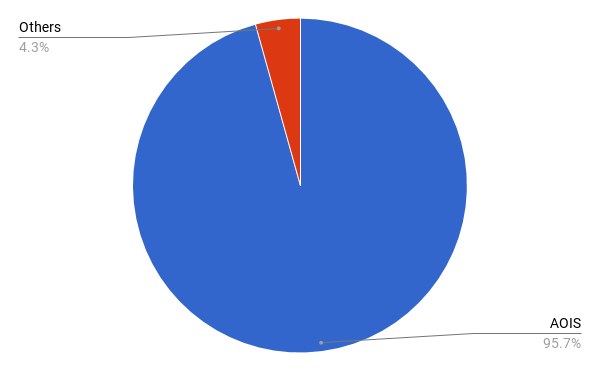
\includegraphics[scale=0.5]{images/chart-total-rules-equivalent.png}
		\caption{E-Rules that avoided more equivalents mutants.}
		\label{fig:rules-equivalents}
	\end{center}
\end{figure*}

We checked some rules that have not been confirmed by TCE, but was confirmed by the manual analysis.
In all projects TCE did not confirm any duplicated mutant generated by the AORB operator (Arithmetic Operator Replacement). 
For example, given \texttt{(x + 1)}, AORB generated mutants like \texttt{(x * 1)} and \texttt{(x / 1)}. 
Because the bytecodes are different (i.e., \texttt{imul} versus \texttt{idiv}), TCE misses these duplicated mutants. 
On the other hand, regarding the \textit{ant} project, TCE confirmed 95\%, 75\%, 60\%, and 10\% of the duplicated mutants generated by ODL x VDL, ROR x SDL, COI x ROR, and SDL x SDL.

Now we answer the research question related to the overhead of executing our rules with respect to time. 
Table~\ref{tab:execution-time} presents the execution time (in seconds) of the original \mujava{} version and the version embedded with our rules. 
For all systems, our version saved time. 
Although our rules introduce an additional overhead, the payoff amount is higher than 12\% for all projects and reached almost 20\% in two projects. 
Because we generate and compile fewer mutants, we have less I/O operations. 
These operations are more expensive than executing our rules.

\scriptsize
\begin{table}[ht]
\centering
\caption{Execution time of \mujava{} without the rules (original version) and with the rules. The presented numbers represent an average of three executions per project.}
\label{tab:execution-time}
\begin{tabular}{|l|r|r|r|}
\hline
\multicolumn{1}{|c|}{\textbf{Project}} & \multicolumn{1}{c|}{\textbf{\mujava{}  w/o Rules}} & \multicolumn{1}{c|}{\textbf{\mujava{} w/ Rules}} & \multicolumn{1}{c|}{\textbf{Difference}} \\
\hline
ant                                            & 871.57s                                                   & 745.84s                                                 & 14.43\%                                          \\ \hline
bcel                                           & 2,345.78s                                                 & 1,888.22s                                               & 19.51\%                                          \\ \hline
commons-lang                                   & 5,235.71s                                                 & 4,189.41s                                               & 19.98\%                                          \\ \hline
commons-math                                   & 430.75s                                                   & 377.3s                                                  & 12.41\%                                          \\ \hline
h2                                             & 8,097.39s                                                 & 6,680.4s                                                & 17.50\%                                          \\ \hline
joda-time                                      & 421.51s                                                   & 368.64s                                                 & 12.54\%                                          \\ \hline
\end{tabular}
\end{table}
\normalsize


\subsection{Threats to Validity}

The projects we used represents a threat to external validity. 
To alleviate this threat, we selected projects of different sizes and domains. 
Also, these projects have been used by the mutation testing community~\cite{KINTIS:2017:1, MADEYISKI:2014:1, KINTIS:2015:1}.

Our rules implementation in \mujava{} is a threat to internal validity. 
We minimize this threat because the majority of the useless mutants have been confirmed as useless by the TCE tool. 
For the remaining ones, we manually analyzed a sample of 10\% of the useless mutants identified by each rule. 
We found a few bugs in our implementation, fixed them, and re-executed the entire analysis. 
In this context, the manual analysis also represents a threat. 
We alleviate such a threat by double checking the questionable cases with a second researcher. 
Additionally, the sample represents a threat as well. 
Nevertheless, we tried to minimize this threat by sampling useless mutants identified by all rules we have implemented.

Our rules can avoid the generation of useless mutants. 
In this way, we can reduce costs not only regarding the generation itself but also on the following two tasks: compiling the useless mutants and executing the test suite against them. 
The execution time we present in Table~\ref{tab:execution-time} confirms the costs reduction. 
The calculation of the execution time also poses an internal threat since the number of I/O tasks is usually high for this type of system. 
So we tried to minimize this threat by running each project three times in each version of \mujava{} and getting the average time.

It is easy to reason about the execution time results, given that we implemented our rules by using a set of conditionals. 
So, the cost of executing a rule should not be higher than generating a mutant and compiling it. 
However, it is important to remember that we have not implemented more costly rules, e.g., the ones that need \textit{def-use} analyses. 
This is a threat to conclusion validity, given that the differences presented in the Table~\ref{tab:execution-time} can change in case we consider such rules 

%However, there is a threat to conclusion validity: these numbers do not consider rules that need \textit{def-use} analyses. 
%So, the differences presented in the table can change in case we consider such rules.


%\section{Better Discussion (RESULTS)}

%\section{Next Steps: Custo/Trade-Off, Comparing with other tools like TCE}

\section{Research Status}
In this chapter, we have demonstrated that the rules can be feasible.
Next, we list the tasks to improve this part of the research.

\begin{enumerate}
    \item \textbf{Improve the result analysis:}~We checked which rules the TCE was able to confirm in the ANT project, but we did not check the reasons that led it to confirm or not a mutant as useless. A special case we identified were the D-Rules AORB x ODL and AORB x AORB that involved the generation of different bytecodes, as explained earlier in this chapter. Further analysis of the mutants confirmed and not confirmed by the TCE will help to understand the limitations of each approach.
    \item \textbf{Implement and evaluate the rules in other mutation testing tools: }~In this work we selected \mujava{} to implement and evaluate our rules. Nevertheless, other mutation tools can also benefit from using the rules and thus avoid useless mutants. This is the case of \pit{}, where we found rules associated with its mutation operators.
    \item \textbf{Compare with other solutions:}~In the evaluation we used TCE just to validate our rules. However, it can also be used as a solution to detect equivalent and duplicated mutants. This way, after implementing a substantial number of rules in \mujava{} we can compare our technique with TCE in terms of performance to reduce the number of useless mutants and calculate the associated cost of each solution. One solution does not subsume the other, given that we can use them in combination. Besides TCE, we intend to investigate other solutions that tackle the equivalent and duplicated mutant problems and compare with our rules.
\end{enumerate}

\chapter{Implications for Practice}
\label{chp:implications}

The high cost of mutation testing is well known. 
Our rules can contribute to the development of better tools and to decrease costs in mutation testing analysis. 
In the end, users can benefit from mutation tools that generate less useless mutants.

In addition, as programming languages evolve, new constructs are added, e.g., Java lambda. 
In this way, developers of mutation testing tools tend (i) to create new mutation operators to cover these new language constructs and (ii) to evolve the existing operators. 
Therefore, they could use our strategy to derive and implement rules to deal with both situations. 
Thus, before releasing the tool, developers can improve confidence that the new version can avoid useless mutants when considering the new operators and the evolved ones. 
However, differently from our evaluation, developers would focus on specific operators (not all available in the tool), reducing costs on carrying out our strategy.

Besides new constructs, the mutation system developer can use the strategy to check if the transformation for a specific mutation operator is working as expected with a wide range of programs. 
During the experiment, our strategy found transformation bugs in \mujava{} and \pit{} that were reported to the respective developers.

%\todo{Leo, precisamos pensar e adicionar mais coisas aqui!}


\chapter{Related Work}
\label{chp:related}

Addressing the equivalent mutant is not a recent problem. Baldwin and Sayward investigated some heuristics for determining equivalence of program mutations~\cite{BALDWIN:1979:1}. Previous works have been addressing this problem and surveys on this topic have been published~\cite{JIA:2011:1, MADEYISKI:2014:1}. The duplicated mutant problem is more recent, but has also been faced~\cite{PAPADAKIS:2015:1, KINTIS:2017:1}.

%A lot of previous works have been fighting this problem. A good synthesis can be found in the surveys of \cite{JIA:2011:1} and \cite{MADEYISKI:2014:1}. The duplicated mutant is a more recent problem, but has also been faced \cite{PAPADAKIS:2015:1, KINTIS:2017:1}. In this section we present previous works about those problems.

To tackle the equivalent mutant problem, researchers used compiler optimizations~\cite{BALDWIN:1979:1}. The intuition is that code optimization can make the original program and the mutant compiled object codes identical. Kintis et al. \cite{KINTIS:2017:1} developed the Trivial Compiler Equivalence (TCE) and used this idea in popular languages (C and Java) and mutation tools (\textsc{Milu} and \mujava{}). In our work, we selected the same Java projects to evaluate our rules. We also used \mujava{}. However, we implemented our own \mujava{} version and selected all available mutation operators. In addition, by using our strategy, we derived rules capable of identifying useless mutants that TCE could not detect.

%In our work we got the same subjects of the aforementioned study and the same mutation testing tool for Java (\mujava{}). However, we used a different version of \mujava{} and selected more mutation operators. Thus, is not fair compare results. But, as can be seen in section \ref{sec:evaluation} our strategy have found mutants that TCE tool did not.

%The first idea to tackle the mutant equivalence was suggested by Baldwin and Sayward \cite{BALDWIN:1979:1} through compiler optimization. The main intuition is that code optimization can transform the mutant and the original program in a way which their compiled object codes will be identical. Kintis at. al \cite{KINTIS:2017:1} developed TCE and experimented this idea in popular languages and mutation tools. 

Offut and Pan~\cite{OFFUT:1996:1, OFFUT:1997:1} developed a technique to detect equivalent mutants based on mathematical constraints that introduce a set of strategies to formulate the killing conditions of the mutants. If these conditions are not feasible, the mutant is equivalent. Voas and McGraw~\cite{VOAS:1997:1} first, and Hierons et al. \cite{HIERONS:1999:1} afterwards, suggested to use program slicing to help with equivalence identification. These approaches suffer from inherent limitations in scalability of the constraint handling and slicing technology. We should have the same scalability problem in case we implement the rules that need \textit{def-use} analyses. Other studies check the impact of mutant execution and suggest non-equivalent mutants. Grun et al.~\cite{GRUN:2009:1} and Shuller and Zeller~\cite{SHULER:2010:1, SHULER:2013:1} proposed that changes in coverage can be used to detect non-equivalents mutants. Shuler et al. \cite{SHULER:2009:1} used invariants violation as a way to classify killable mutants. Regarding duplicated mutants detection, little effort has been spent on this front~\cite{PAPADAKIS:2015:1, KINTIS:2017:1}. All these aforementioned works require the generation, compilation, and analysis of the mutants to identify the useless ones. Differently, our rules are applied at the mutant generation moment, which means that the useless mutants would not be generated at all.

Kintis and Malevris~\cite{KINTIS:2015:1} also avoid the equivalent mutants generation. To do so, they rely on static analysis tools. They introduce data-flow patterns and showed that a large portion of equivalent mutants can be avoided by just analyzing the original program under test. The idea of the data-flow patterns is similar to our rules. We have rules that depend on AST traversal and \textit{def-use} analyses. However, we have rules to detect duplicated mutants. In addition, we also propose a strategy to help with the task of deriving new rules. Developers of mutation testing tools can use our strategy to help them with deriving new rules and thus release better tools.

Just et. al~\cite{JUST:2017:1} criticize the strategies based on reducing the number of applied mutation operators because they might work in a set of programs but not in another set. This way, depending on the program, these strategies continue to generate a high number of useless mutants. The authors conclude that, to discard some of the mutation operators, we need to first understand the program constructs to which the operators will be applied. In our work, we follow this rationale. We do not remove the mutation operators entirely to reduce costs. Rather, we can use all operators, but we avoid specific transformations defined in each rule.


\section{Research Status}
Here we list our improvements for Related Work section.

\begin{enumerate}
    \item We plan to extend this chapter with related work that has not been published yet or that we eventually bypassed during our research.
\end{enumerate}



%\section{Introduction}

%\section{Better Discussion (RESULTS)}

%\section{Next Steps: Custo/Trade-Off, Comparing with other tools like TCE}

\chapter{Concluding Remarks}

In this work, we introduced a strategy to help to identify rules to avoid useless mutants, i.e., equivalent and duplicated mutants. 
As input, we pass a set of programs. 
For each program \textit{P}, the strategy also needs a passing test suite and a set of mutants derived from \textit{P}. 
As output, our strategy yields a set of useless mutants candidates. 
To evaluate the strategy, we used 4,999 mutants. 
The strategy classified 963 as equivalent and 1,332 as duplicated. 
By carefully analyzing this output, we derived \NumberOfNewHeuristics new rules. 

Because we derived the rules by using artificial and small Java programs, we decided to implement a subset of our rules in the \mujava{} mutation tool to check whether our rules can identify useless mutants in industrial-scale projects. 
By using well-known open-source projects, we could avoid the generation of almost 13\% of useless mutants, on average. 
This result is relatively low when compared to related work, but it is promising because, instead of generating and checking whether the mutants are indeed useless, we do not generate the useless mutants at all. 
In addition, we can derive and implement more rules in case we set our strategy to use more complex programs.

To understand the overhead brought by our technique, we executed the new \mujava{} version embedded with \NumberOfImplementedHeuristics rules in the same industrial-scale systems and compared against the original \mujava{} version.
In spite of the additional overhead, the new \mujava{} version had a payoff higher than 12\% for all projects and reached almost 20\% in two projects. 

Our technique does not eliminate other solutions that detect mutants after their generation. 
Therefore we believe that combining two or more techniques may increase the adoption of mutation testing by the industry.

%To derive more rules, as future work we intend to set our strategy to use different Java programs and different test suite generators (e.g., EvoSuite~\cite{FRASER:2011:1}). In addition, we intend to implement the rules that need \textit{def-use} analyses and evaluate their overhead. 
%Last but not least, we should implement our rules in different mutation testing tools (e.g., \pit{}).

%\section{Limitations}

\section{Research Status}
In this section, we present the schedule of the planned activities for the remaining work of this thesis, discussed in the research status sections throughout the text.
Figure \ref{fig:summary-next-steps} summarizes our planned schedule for the next 18 months. 


\begin{figure}[ht]
	\begin{center}
		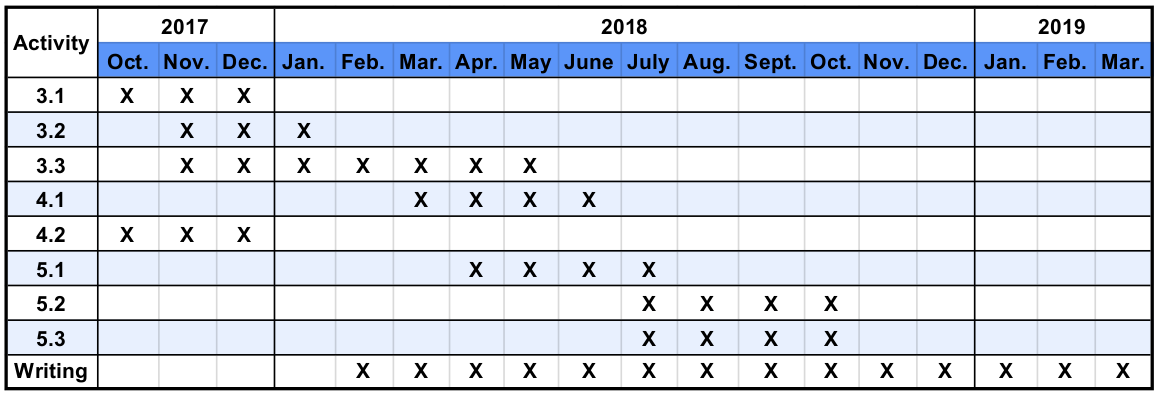
\includegraphics[scale=0.40]{images/Summary-Next-Steps.png}
		\caption{Schedule.}
		\label{fig:summary-next-steps}
	\end{center}
\end{figure}

We use, for example, 3.1 to denote the first item enumerated in the Research Status section of Chapter~\ref{sec:strategy} and so forth. 
The planned activities of the chapters not listed in Figure \ref{fig:summary-next-steps} are included in the writing activity.
% \chapter{Next Steps}
\label{sec:nextsteps}

In the Chapters 

\section{Mind Map}

\section{Time Table}


\backmatter

% Appendix
\appendix
\chapter{List of Rules}
\label{ap:list-rules}
In this appendix, we list the new rules identified.
In Section \ref{sec:examples-of-rules} we have presented nine rules. 
We now present the remaining 28.

\section{E-Rules}

\\
\\
% \textbf{E-Rule. PNC}~(\mujava{})\\
% $term = new~C().v $\\
% $transformations = \{ \\ \indent PNC(C, D)~=~D \\ \}$\\
% $constraints = \{$ \\ \indent $D$~extends~$C$, \\ \indent $v$~exists only in$~C$, \\ \indent $D$~constructor does not change$~v$, \\ \indent $D$~constructor calls the same~$C$~constructor \\ \}$ $\\
% \\
% \\
% \textbf{E-Rule. ISD}~(\mujava{})\\
% $term = super.v$\\
% $transformations = \{\\ \indent ISD(super.v) =~v \\\}$\\
% $constraints = \{ \\ \indent v$~exists~only~in~superclasses \\ $\}$\\
% \\
% \\
% \textbf{E-Rule. JID}~(\mujava{})\\
% $term = v~:=~value$\\
% $transformations = \{\\ \indent JID(value) =~; \\\}$\\
% $constraints = \{ \\ \indent value$~assigned~to~$v$~is the default value of the type of $v$ \\ $\}$\\
% \\
% \\
% \textbf{E-Rule. AOIS-01}~(\mujava{})\\
% $term = v~:=~v~op1~exp$\\
% $transformations = \{\\ \indent AOIS(v,~op2)~=~v~op2; \\\}$\\
% $constraints = \{ $\\ 
% \indent the use of~$v$~is the last one in the RHS, \\ 
% \indent $op2 \in \{++, --\} \\ \}$\\
% \\
% \\
% \textbf{E-Rule. AOIS-02}~(\mujava{})\\
% $term = v$\\
% $transformations = \{\\ \indent AOIS(v,~op)~=~v~op; \\\}$\\
% $constraints = \{ \\$ 
% \indent $v$ has a local scope, \\ 
% \indent the use of~$v$~is the last one in its scope,  \\ 
% \indent $op~\in~\{++,~--\}$ \\ 
% \}\\
% \\
% \\
% \textbf{E-Rule. ROR}*~(\mujava{})\\
% $term = if~(exp1~op1~exp2){~return~exp1~}~else~{~return~exp2~}$\\
% $transformations = \{\\ \indent ROR(op1,~op2)~=~op2; \\\}$\\
% $constraints = \{ \\$ 
% \indent $op1~\in \{>\}$ and $op2~\in \{>=\}$ or \\ 
% \indent $op1~\in \{<\}$ and $op2~\in \{<=\}$ \\  \}\\
% \\
% *This rule also occur in ROR~(\major{}) and ConditionalBoundary~(\pit{}).
% \\
% \\
\textbf{E-Rule. JSI}~(\mujava{})\\
$term = type~v~:=~value$\\
$transformations = \{\\ \indent JSI(type v)~=~static~type~v; \\\}$\\
$constraints = \{ \\$ 
\indent $v$ is read-only\\  \}\\

% \textbf{E-Rule. MemberVariable}~(\pit{})\\
% $term = v~:=~value$\\
% $transformations = \{\\ \indent MemberVariable(value)~=~; \\\}$\\
% $constraints = \{ \\$ 
% \indent value assigned to $v$ is the default value for the type of $v$\\  \}\\
% \\
% \\

%-----------------------------------------------------


\section{D-Rules}

% \textbf{D-Rule. ODL x VDL}~(\mujava{})\\
% $term = exp~op~v $\\
% $transformations = \{\\ \indent ODL(exp~op~v) = exp,\\ \indent VDL(exp~op~v) = exp\\\}$\\
% \\
% \\
% \textbf{D-Rule. ROR x SDL}~(\mujava{})\\
% $term = if~(exp_1~op~exp_2)~\{b\} $\\
% $transformations = \{\\ \indent ROR(exp_1~op~exp_2) = false, \\ \indent SDL(if~(exp_1~op~exp_2)~\{b\}) =~; \\ \}$\\
% \\
% \\
% \textbf{D-Rule. LOI x LOD}~(\mujava{})\\
% $term = {\sim}v$\\
% $transformations = \{\\ \indent LOI(v) = {\sim\sim} v,\\ \indent LOD({\sim}v) = v \\\}$\\
% \\
% \\
% \textbf{D-Rule. SDL x SDL}~(\mujava{})\\
% $term = if~(exp)~{~s~} $\\
% $transformations = \{\\ \indent SDL(s) =~;, \\ \indent SDL(if~(exp)~s) =~; \\ \}$\\
% $constraints = \{\\$ \indent $exp$~has~no~side~effect $\\\}$\\
% \\
% \\
% \textbf{D-Rule. AOR x LVR}~(\major{})\\
% $term =  exp~op_1~1 $\\
% $transformations = \{ \\ \indent AOR(exp~op_1~1,~op_2) = exp~op_2~1, \\
% \indent LVR(1)=0 \\ \}$\\
% $constraints = \{\\ \indent op_1~\in~\{+, -\}~, \\ \indent op_2~\in~\{*, /\} \\ \}$\\
% \\
% \\
% \textbf{D-Rule. InlineConstant x RemoveConditionals}~(\pit{})\\
% $term = if~(exp)~{~v~:=~v~op~1} $\\
% $transformations = \{ \\ \indent InlineConstant(1)~=~0,\\ \indent RemoveConditionals(exp)=false \\ \}$\\
% $constraints = \{ \\$ \indent $op~\in~\{+, -\}$, \\ \indent $exp$~has~no~side~effect $ \\ \}$
% \\
% \\
% \textbf{D-Rule. AODU x AOIU}~(\mujava{})\\
% $term = v~:=~-exp;~b;~return~v$\\
% $transformations = \{ \\ \indent AODU(-exp)~=~exp,\\ \indent AOIU(v)~=~-v \\ \}$\\
% $constraints = \{ \\$ 
% \indent there is no definition and use of $v$ in $b$, \\ 
% \indent $v$ has local scope\\
% \}\\
% \\
% \\
% \textbf{D-Rule. LOI x LOI-01}~(\mujava{})\\
% $term = v1 := v2; b; return~v1$\\
% $transformations = \{\\ \indent LOI(v2) = {\sim} v2,\\ \indent LOI(v1) = {\sim} v1$\\\}\\
% $constraints = \{\\$ 
% \indent there is no definition and use of $v1$ in $b$, \\
% \indent $v1$ has local scope \\
% \}
% \\
% \\
\textbf{D-Rule. SDL x VDL}~(\mujava{})\\
$term = v~op; $\\
$transformations = \{\\ \indent SDL(v~op)~=~;,\\ \indent VDL(v~op)~=~;\\\}$\\
$constraints = \{ \\$ \indent $op~\in~\{++, --\}  \\ \}$
\\
\\
\textbf{D-Rule. SDL x ODL}~(\mujava{})\\
$term = v~:=~v~op~exp $\\
$transformations = \{\\ \indent SDL(v~:=~v~op~exp)~=~;,\\ \indent ODL(op~exp)~=~;\\\}$\\
$constraints = \{ \\$ \indent $op$ is any binary (infix) operator $\\ \}$
\\
\\
\textbf{D-Rule. ODL x AODS}~(\mujava{})\\
$term = op~v $\\
$transformations = \{\\ \indent ODL(v~op)~=~v,\\ \indent AODS(op)~=~;\\\}$\\
$constraints = \{ \\$ \indent $op~\in~\{++, --\}  \\ \}$
\\
\\
% \textbf{D-Rule. LOI x LOI-2}~(\mujava{})\\
% $term = if~(v1~op~v2) $\\
% $transformations = \{\\ \indent LOI(v2) = {\sim} v2,\\ \indent LOI(v1) = {\sim} v1$\\\}\\
% $constraints = \{ \\$ \indent $op~\in~\{==, !=\}  \\ \}$
% \\
% \\
% \textbf{D-Rule. ODL x ODL}~(\mujava{})\\
% $term = exp1~op~exp2 $\\
% $transformations = \{\\ \indent ODL(exp1~op~exp2) = exp1,\\ \indent ODL(exp1~op~exp2) = exp2$\\\}\\
% $constraints = \{ \\ \indent exp1$ is equal to $exp2 \\ \}$
% \\
% \\
\textbf{D-Rule. IOD x ISI}~(\mujava{})\\
$term = type f1()\{~f2()]~\};~type~f2()\{~\}; $\\
$transformations = \{\\ \indent IOD(type~f2(){~}) = ;,\\ \indent ISI(f2()) = super.f2()$\\\}\\
$constraints = \{ \\ \indent type~f2(){ }$ must overwriting $f2$ from superclass $\\ \}$
\\
\\
\textbf{D-Rule. CDL x ODL}~(\mujava{})\\
$term = exp~op~c $\\
$transformations = \{\\ \indent CDL(c) = ;,\\ \indent ODL(exp~op~c) = exp$\\\}\\
\\
\\
\textbf{D-Rule. AODU x ODL}~(\mujava{})\\
$term = op~exp $\\
$transformations = \{\\ \indent AODU(op) = ;,\\ \indent ODL(op~exp) = exp$\\\}\\
$constraints = \{ \\$ \indent $op~\in~\{+, -\}  \\ \}$
\\
\\
\textbf{D-Rule. COD x ODL}~(\mujava{})\\
$term = !~exp $\\
$transformations = \{\\ \indent COD(!) = ;,\\ \indent ODL(!~exp) = exp$\\\}\\
\\
\\
\textbf{D-Rule. LOD x ODL}~(\mujava{})\\
$term = {\sim}exp $\\
$transformations = \{\\ \indent LOD({\sim}) = ;,\\ \indent ODL({\sim}exp) = exp$\\\}\\
\\
\\
\textbf{D-Rule. COI x ROR}~(\mujava{})\\
$term = (exp1~op1~exp2) $\\
$transformations = \{\\ \indent COI(exp1~op1~exp2)~=~!(exp1~op1~exp2),\\ \indent ROR(op1)~=~op2$\\\}\\
$constraints = \{ \\$ 
\indent $op1~\in~\{>\}$ and $ op2~\in~\{<=\}~or~ $\\
\indent $op1~\in~\{<\}$ and $ op2~\in~\{>=\}~or~  $\\ 
\indent $op1~\in~\{>=\}$ and $ op2~\in~\{>\}~or~  $\\ 
\indent $op1~\in~\{<=\}$ and $ op2~\in~\{<\}~or~  $\\ 
\indent $op1~\in~\{==\}$ and $ op2~\in~\{!=\}~or~  $\\ 
\indent $op1~\in~\{!=\}$ and $ op2~\in~\{==\}  $\\ 
$\}$
\\
\\
\textbf{D-Rule. COD x ROR}~(\mujava{})\\
$term = !(exp1~op1~exp2) $\\
$transformations = \{\\ \indent COD(!)~=~;,\\ \indent ROR(op1)~=~op2$\\\}\\
$constraints = \{ \\$ 
\indent $op1~\in~\{>\}$ and $ op2~\in~\{<=\}~or~ $\\
\indent $op1~\in~\{<\}$ and $ op2~\in~\{>=\}~or~  $\\ 
\indent $op1~\in~\{>=\}$ and $ op2~\in~\{>\}~or~  $\\ 
\indent $op1~\in~\{<=\}$ and $ op2~\in~\{<\}~or~  $\\ 
\indent $op1~\in~\{==\}$ and $ op2~\in~\{!=\}~or~  $\\ 
\indent $op1~\in~\{!=\}$ and $ op2~\in~\{==\}  $\\ 
$\}$
\\
\\
\textbf{D-Rule. AORS x ODL}~(\mujava{})\\
$term = return~op1~v) $\\
$transformations = \{\\ \indent AORS(op1~v)~=~v~op2;,\\ \indent ODL(op1~v)~=~v$\\\}\\
$constraints = \{ \\$ 
\indent $v$ has a local scope, \\
\indent the use of $v$ is the last one in its scope \\
\indent $op1$ is pre-increment or pre-decrement, \\ 
\indent $op2$ is post-increment or post-decrement \\ 
$\}$
\\
\\
\textbf{D-Rule. AORB x ODL}~(\mujava{})\\
$term = exp~op1~1 $\\
$transformations = \{\\ \indent AORB(op1)~=~op2,\\ \indent ODL(exp~op1~1)~=~exp$\\\}\\
$constraints = \{ \\$ 
\indent $op1~\in~\{+, -\}$  \\
\indent $op2~\in~\{*, /\}$  \\ 
$\}$
\\
\\
% \textbf{D-Rule. AOIS x AOIS}~(\mujava{})\\
% $term = v1~:=~v2;~b;~v3~:=~v2 $\\
% $transformations = \{\\ \indent AOIS(v2, op1)~=~v2~op1;,\\ \indent AOIS(v2, op2)~=~op2~v2$\\\}\\
% $constraints = \{ \\$ 
% \indent there is no definition of $v2$ in $b$, \\
% \indent $op1$ is post-increment and op2 is pre-increment operator or \\ 
% \indent $op1$ is post-decrement and op2 is pre-decrement operator \\ 
% $\}$
% \\
% \\
\textbf{D-Rule. AOBR x AORB}~(\mujava{})\\
$term = v~op1~1 $\\
$transformations = \{\\ \indent AORB(op1, op2)~=~op2,\\ \indent AORB(op1, op3)~=~op3$\\\}\\
$constraints = \{ \\$ 
\indent $op1~\in~\{+, -\},  $\\
\indent $op2$ and $op3~\in~\{*, /\}  $\\ 
$\}$
\\
\\
% \textbf{D-Rule. AOIU x AODU}~(\mujava{})\\
% $term = v1~:=~-exp;~b;~return~v1 $\\
% $transformations = \{\\ \indent AOIU(v1)~=~-v1,\\ \indent AODU(-exp)~=~exp$\\\}\\
% $constraints = \{ \\$ 
% \indent there is no definition of $v1$ in $b$,  \\
% \indent $v1$ has a local scope \\ 
% $\}$
% \\
% \\
\textbf{D-Rule. AORS x LOI}~(\mujava{})\\
$term = v~op1 $\\
$transformations = \{\\ \indent AORS(v~op1, op2)~=~op2~v,\\ \indent LOI(v)~=~{\sim}v$\\\}\\
$constraints = \{ \\$ 
\indent $op1~\in~\{++\}  $\\ 
\indent $op2~\in~\{--\}  $\\ 
\indent $v$ must start with zero \\ 
\indent the only definition of $v$ in the program is in this line line of the $term$\\ 
$\}$
\\
\\
\textbf{D-Rule. AORS x AOIU}~(\mujava{})\\
$term = v~op1 $\\
$transformations = \{\\ \indent AORS(v~op1, op2)~=~v~op2,\\ \indent AOIU(v)~=~-v$\\\}\\
$constraints = \{ \\$ 
\indent $op1~\in~\{++\}  $\\ 
\indent $op2~\in~\{--\}  $\\ 
\indent $v$ must start with zero \\ 
\indent the only definition of $v$ in the program is in this line line of the $term$\\ 
$\}$
\\
\\
\textbf{D-Rule. ODL x LOI}~(\mujava{})\\
$term = v1~:=~{\sim}exp;~b;~return~v1 $\\
$transformations = \{\\ \indent ODL({\sim}exp)~=~exp,\\ \indent LOI(v1)~=~{\sim}v1$\\\}\\
$constraints = \{ \\$ 
\indent there is no definition of $v1$ in $b$, \\ 
\indent $v1$ has a local scope \\ 
$\}$
\\
\\
\textbf{D-Rule. AOIS x CDL}~(\mujava{})\\
$term = return~v~op1~1 $\\
$transformations = \{\\ \indent AOIS(v,~op2)~=~op2~v,\\ \indent CDL(1)~=~;$\\\}\\
$constraints = \{ \\$ 
\indent $op1~\in~\{+\} $ and $op2~\in~\{--\}$, \\ 
\indent $op1~\in~\{-\} $ and $op2~\in~\{++\}$, \\ 
\indent $v$ has a local scope, \\ 
\indent the use of~$v$~is the last one in its scope \\ 
$\}$
\\
\\
\textbf{D-Rule. ORU x STD}~(\major{})\\
$term = v~:=~-v $\\
$transformations = \{\\ \indent ORU(-)~=~+,\\ \indent STD(v~:=~-v)~=~;$\\\}\\
\\
\\
\textbf{D-Rule. InlineConstant x MemberVariable}~(\pit{})\\
$term = v~:=~v~op~1 $\\
$transformations = \{\\ \indent InlineConstant(1)~=~0,\\ \indent MemberVariable(v~:=~v~op~1)~=~;$\\\}\\
$constraints = \{ \\$ 
\indent $op~\in~\{+, -\} $\\ 
$\}$
\\
\\
\textbf{D-Rule. InlineConstant x Math}*~(\pit{})\\
$term = {\sim}v $\\
$transformations = \{\\ 
\indent InlineConstant({\sim}v)~=~v~\hat{~}~0x0,\\ 
\indent Math({\sim}v)~=~v~\&~0xFFFFFFF$\\ \}\\
$constraints = \{ \\$ 
\indent $op~\in~\{+, -\} $\\ 
$\}$\\
* in byte code: ${\sim}v == v~\hat{~}~0xFFFFFFFF$
\\
\\
\textbf{D-Rule. ReturnVals x NonVoidMethodCal}~(\pit{})\\
$term = type~f1(){~b;~return~exp~};type~f2(){~v~:=~f1()~}$\\
$transformations = \{\\ 
\indent ReturnVals(return~exp)~=~return~defaultValue,\\ 
\indent NonVoidMethodCal(~v~:=~f1()~)~=~v~:=~defaultValue~$\\\}\\
$constraints = \{ \\$ 
\indent the function $f1()$ has not side effect, \\ 
\indent there is only one return in $f1()$, \\
\indent there is no other place that calls $f1()$, \\ 
$\}$\\
\\
\\
\textbf{D-Rule. NonVoidMethodCall x InlineConstant}~(\pit{})\\
$term = v~:=~f()~op~c $\\
$transformations = \{\\ 
\indent NonVoidMethodCall(~f()~)~=~defaultValue,\\ 
\indent InlineConstant(~c~)~=~0$\\\}\\
$constraints = \{ \\$ 
\indent $op~\in~\{*\}$, \\ 
\indent $f()$ can be any primitive numeric type \\
$\}$\\
\\
\\
\textbf{D-Rule. InlineConstant x ReturnVals}~(\pit{})\\
$term = v~:=~c;~b;~return~v $\\
$transformations = \{\\ 
\indent InlineConstant(~c~)~=~0,\\ 
\indent ReturnVals(~return~v~)~=~return~defaultValue$\\\}\\
$constraints = \{ \\$ 
\indent there is no definition of $v$ in $b$, \\ 
\indent $v$ can be any primitive numeric type, \\
\indent there is only one path from $v~:=~c$ to $return~v$ \\
$\}$\\
\\
\\
\textbf{D-Rule. MemberVariable x ReturnVals}~(\pit{})\\
$term = type~v~:=~c;~type~f(){~return~v~} $\\
$transformations = \{\\ 
\indent MemberVariable(~type~v~:=~c~)~=~type~v~:=~defaultValue,\\ 
\indent ReturnVals(~return~v~)~=~return~defaultValue$\\\}\\
$constraints = \{ \\$ 
\indent $v$ has only one point of definition, \\
\indent $v$ has only one point of use \\
$\}$\\
\\
\\
\textbf{D-Rule. MemberVariable x RemoverConditional\_EQUAL\_ELSE}~(\pit{})\\
$term = if(exp){~v~:=~exp~}$\\
$transformations = \{\\ 
\indent MemberVariable(~v~:=~exp~)~=~;,\\ 
\indent RemoverConditional\_EQUAL\_ELSE(~if(exp)~)~=~if(false)$\\\}\\
$constraints = \{ \\$ 
\indent there is no else statements, \\ 
\indent if expression has no side effect \\
$\}$\\
\\
\\
% \textbf{D-Rule. MemberVariable x RemoverConditional\_EQUAL\_ELSE}~(\pit{})\\
% $term = if(exp){~v~:=~exp~}$\\
% $transformations = \{\\ 
% \indent MemberVariable(~v~:=~exp~)~=~;,\\ 
% \indent RemoverConditional\_EQUAL\_ELSE(~if(exp)~)~=~if(false)$\\\}\\
% $constraints = \{ \\$ 
% \indent there is no else statements, \\ 
% \indent if expression has no side effect \\
% $\}$\\
% \\
% \\
\textbf{D-Rule. MemberVariable x Math}*~(\pit{})\\
$term = {\sim}v $\\
$transformations = \{\\ 
\indent MemberVariable(v)~=~{\sim}v,\\ 
\indent Math({\sim}v)~=~v~\&~0xFFFFFFF$\\ \}\\
* in byte code: ${\sim}v == v~\hat{~}~0xFFFFFFFF$
\\
\\
\textbf{D-Rule. InvertNegs x MemberVariable}~(\pit{})\\
$term = v~:=~-v~$\\
$transformations = \{\\ 
\indent InvertNegs(-v)~=~v,\\ 
\indent MemberVariable(~v~:=~-v~)~=~;$\\\}\\
\\
\\
% \textbf{D-Rule. InlineConstant x RemoverConditional\_EQUAL\_ELSE}~(\pit{})\\
% $term = if(exp)~v~:=~v~op1~$\\
% $transformations = \{\\ 
% \indent InlineConstant(~1~)~=~0,\\ 
% \indent RemoverConditional\_EQUAL\_ELSE(~if(exp)~)~=~if(false)$\\\}\\
% $constraints = \{ \\$ 
% \indent $op~\in~\{+. -\}$, \\ 
% \indent $exp$ has no side effect \\
% $\}$\\





% \begin{table}[htp]
	\caption{List of journals in which the searches were performed.}
	\label{tbl:journals_list}
	\centering
	\rowcolors{2}{lightgray!30}{white}
	\begin{tabular}{l}
	\toprule
	\textbf{Journal title} \\
	\toprule
	ACM Transactions on Software Engineering and Methodology \\
	Automated Software Engineering \\
	Elsevier Information and Software Technology \\
	Elsevier Journal of Systems and Software \\
	Empirical Software Engineering \\
	IEEE Software \\
	IEEE Computer \\
	IEEE Transactions on Software Engineering \\
	International Journal of Software Engineering and Knowledge Engineering \\
	Journal of Software: Evolution and Process \\
	Software Quality Journal \\
	Journal of Software \\
	Software Practice and Experience Journal \\
	\bottomrule
	\end{tabular}
\end{table}

% References
\bibliographystyle{plain}
%\begin{references}
\bibliography{references}
%\end{references}



% Cзlofon
% Inclui uma pequena nota com referЖncia Я UFPEThesis
% Comente para omitir
\colophon


\end{document}
